\documentclass[sigconf, nonacm]{acmart}
\usepackage{amsmath,amsfonts}
\usepackage{algorithm}
\usepackage{algorithmicx}
\usepackage{algpseudocode}
\usepackage{graphicx}
\usepackage{textcomp}
\usepackage{listings}
\usepackage{xcolor}
\usepackage[english]{babel}
\usepackage{color,colortbl}
\usepackage{xspace}
\usepackage{multirow}
\usepackage{graphicx}
\usepackage{booktabs}
\usepackage{url}
\usepackage{xurl}
\usepackage{tipa}
% \usepackage{minted}
\usepackage[T1]{fontenc}
\usepackage[utf8]{inputenc}
% \usepackage{scrlayer-scrpage}
\usepackage{threeparttable}
% \usepackage{balance}
\usepackage{amsmath,amsfonts}
\usepackage{pifont}
% \usepackage{fontspec}
% \usepackage{libertine}
\usepackage{tabularx}
\usepackage[printonlyused]{acronym}
\usepackage[most]{tcolorbox}

\usepackage{hyperref}
\hypersetup{
	pdftitle={},
	pdfauthor={},
	pdfsubject={},
	pdfkeywords={},
	bookmarksnumbered=true,
	bookmarksopen=false,
	colorlinks=true,
	pdfstartview=FitB,
	pdfpagemode=UseOutlines
}


\definecolor{background}{HTML}{EEEEEE}
% \definecolor{eclipseStrings}{RGB}{42,0.0,255}
% \definecolor{eclipseKeywords}{RGB}{42,0.0,255}
\definecolor{mygreen}{rgb}{0,0.6,0}
\definecolor{mygray}{rgb}{0.5,0.5,0.5}
\definecolor{mymauve}{rgb}{0.58,0,0.82}


\lstdefinelanguage{json}{
    basicstyle=\footnotesize\ttfamily,
    commentstyle=\color{black}, % style of comment
    stringstyle=\color{black}, % style of strings
    numbers=left,
    numberstyle=\scriptsize,
    stepnumber=1,
    numbersep=8pt,
    showstringspaces=false,
    breaklines=true,
    frame=lines,
    backgroundcolor=\color{background}, %only if you like
    string=[s]{"}{"},
    comment=[l]{:\ "},
    morecomment=[l]{:"},
}

%listing set
% \lstset{
%   numbers=none,
%   basicstyle=\small,
%   breaklines=true,
%   columns=flexible
% }

% circle 1~20
\newcommand{\libcirc}[1]{\ding{\numexpr171+#1\relax}}

% tikz
\usepackage{tikz}
\usetikzlibrary{shapes,arrows,positioning,fit}
\usetikzlibrary{backgrounds}

% \pdfsuppresswarningpagegroup=1


\lstset{ %
	backgroundcolor=\color{white},   % choose the background color
	basicstyle=\footnotesize\ttfamily, % size of fonts used for the code
	breaklines=true,                 % automatic line breaking only at whitespace
	captionpos=b,                    % sets the caption-position to bottom
	commentstyle=\color{mygreen},    % comment style
	escapeinside={\%*}{*)},          % if you want to add LaTeX within your code
	keywordstyle=\color{blue},       % keyword style
	stringstyle=\color{mymauve},     % string literal style
	numbers=left,
	numberstyle=\tiny\ttfamily,
	%	frame=shadowbox,
	rulesepcolor=\color{red!20!green!20!blue!20},
	firstnumber=1,
	showspaces=false,                % show spaces everywhere adding particular underscores; it overrides 'showstringspaces'
	showstringspaces=false,          % underline spaces within strings only
	showtabs=false,
    columns=flexible,
    language=json,
	escapeinside={<@}{@>}            % <@\textcolor{red}{text}@>
}

%\setlength\tabcolsep{2pt}
%\resizebox{\textwidth}{!}{}
%\resizebox{\columnwidth}{!}{}
%\mbox{}
%\setlength{\abovecaptionskip}{0pt}
%\setlength{\belowcaptionskip}{0pt}


%\usepackage[font=footnotesize,skip=0pt,belowskip=0pt,aboveskip=0pt]{caption}
%\captionsetup[table]{format=plain,labelformat=simple,labelsep=period}
\usepackage{caption}
\captionsetup[table]{font=footnotesize,skip=4pt,}
\captionsetup[figure]{font=footnotesize,skip=4pt,}
\captionsetup[figure]{aboveskip=8pt,belowskip=-8pt}

\setlength{\emergencystretch}{40pt}

% for IEEE
% \IEEEoverridecommandlockouts

% for acm template
%\settopmatter{printacmref=false} % Removes citation information below abstract
%\renewcommand\footnotetextcopyrightpermission[1]{} % removes footnote with conference information in first column
%\fancyhf{} % Remove fancy page headers 
%\fancyfoot[C]{\thepage}
%\settopmatter{printacmref=false, printccs=true, printfolios=true} % We want page numbers on submissions

\newcommand{\zhiyun}[1]{\textcolor{blue}{[Zhiyun: #1]}}
\newcommand{\zhiyune}[1]{\textcolor{blue}{[#1]}}
\newcommand{\shitong}[1]{\textcolor{orange}{[Shitong: #1]}}
\newcommand{\guoren}[1]{\textcolor{olive}{[Guoren: #1]}}
\newcommand{\yu}[1]{\textcolor{mygreen}{[Yu: #1]}}
\newcommand{\yutext}[1]{\textcolor{red}{[Yu\_text: #1]}}
% \newcommand{\yu}[1]{}
%\newcommand{\yutext}[1]{#1}
% \newcommand{\haonan}[1]{}
% \newcommand{\zhiyun}[1]{}
\newcommand{\haonan}[1]{\mytodogrey{[haonan: #1]}}
\newcommand{\mytodogrey}[1]{\textcolor{cyan}{\ding{46}~{\sf}~#1}}

\newcommand{\etc}{\textit{etc.}\xspace}
\newcommand{\etal}{\textit{et al.}\xspace}
\newcommand{\ie}{\textit{i.e.,}\xspace}    % in other words
\newcommand{\eg}{\textit{e.g.,}\xspace}    % for example

\newcommand{\squishlist}{
	\begin{list}{$\bullet$} {
			\setlength{\itemsep}{0pt}
			\setlength{\parsep}{0pt}
			\setlength{\topsep}{0pt}
			\setlength{\partopsep}{0pt}
			\setlength{\leftmargin}{1.0em}
			\setlength{\labelwidth}{1em}
			\setlength{\labelsep}{0.5em}
		}
		}
		\newcommand{\squishend}{
	\end{list}
}



\newcommand\graybox[1]{%
\noindent % no intented box !!
\colorbox{gray!20}{\parbox[t]{0.975\linewidth}{%
% \def\insideitemize{itemize}
%  \ifx\@currenvir\insideitemize  
%         \parskip 4pt plus 2pt minus 1pt % like itemsep
%   \else
%         \parindent\currentparindent % use the global indentation
%         \parskip\currentparskip  % use the global paragrapk skip

% \fi
#1}}}

\newcommand{\find}[1]{
\begin{tcolorbox}[leftrule=1mm,rightrule=1mm,toprule=0mm,bottomrule=0mm,left=1pt,right=1pt,top=0.5pt,bottom=0.5pt]
\em #1
\end{tcolorbox}
}

\newcommand{\cut}[1] {}

\cut{\zhiyun{a few things we should do before submission:
		\begin{itemize}
			\item check captilization consistency, ``figure -> Figure'', caption of a figure/table should have the first letter captilized only
			\item center the caption of all figures/tables.
			\item remove the ``period'' mark in captions.
			\item spell check / grammar check (put all sentences in grammarly)
			\item for all the functions referened in textit\{\}, we should add the brackets. For example, ``textit\{fun\} -> textit\{fun()\}''
			\item global replace of ``\ textit'' with ''\ texttt''. Also, there is no need to add the quotation marks around \texttt.
			\item check the text that references the figure and the figure itself are always co-located on the same page (or one page before/after).
		\end{itemize}
	}}

\acmConference[SomeConf ]{xxt  Conference on Something}{Aug 2023}{Earth}

%%
%% \BibTeX command to typeset BibTeX logo in the docs
\AtBeginDocument{%
  \providecommand\BibTeX{{%
    Bib\TeX}}}

%% Rights management information.  This information is sent to you
%% when you complete the rights form.  These commands have SAMPLE
%% values in them; it is your responsibility as an author to replace
%% the commands and values with those provided to you when you
%% complete the rights form.
% \setcopyright{acmcopyright}
% \copyrightyear{2018}
% \acmYear{2018}
% \acmDOI{XXXXXXX.XXXXXXX}

%% These commands are for a PROCEEDINGS abstract or paper.
% \acmConference[Conference acronym 'XX]{Make sure to enter the correct
%   conference title from your rights confirmation emai}{June 03--05,
%   2018}{Woodstock, NY}
%%
%%  Uncomment \acmBooktitle if the title of the proceedings is different
%%  from ``Proceedings of ...''!
%%
%%\acmBooktitle{Woodstock '18: ACM Symposium on Neural Gaze Detection,
%%  June 03--05, 2018, Woodstock, NY}
% \acmPrice{15.00}
% \acmISBN{978-1-4503-XXXX-X/18/06}


\author{Haonan Li}
\email{hli333@ucr.edu}
\affiliation{%
    \institution{UC Riverside}
    \city{Riverside}
    \state{California}
    \country{USA}
}

\author{Yu Hao}
\email{yhao016@ucr.edu}

\affiliation{%
    \institution{UC Riverside}
    \city{Riverside}
    \state{California}
    \country{USA}
}

\author{Yizhuo Zhai}
\email{yzhai003@ucr.edu}

\affiliation{%
    \institution{UC Riverside}
    \city{Riverside}
    \state{California}
    \country{USA}
}

\author{Zhiyun Qian}
\email{zhiyunq@cs.ucr.edu}

\affiliation{%
    \institution{UC Riverside}
    \city{Riverside}
    \state{California}
    \country{USA}
}
%%
%% Submission ID.
%% Use this when submitting an article to a sponsored event. You'll
%% receive a unique submission ID from the organizers
%% of the event, and this ID should be used as the parameter to this command.
%%\acmSubmissionID{123-A56-BU3}


\newcommand{\work}{\mbox{\textsc{LLift}}\xspace}
\newcommand{\PP}[1]{
	\vspace{2px}
	\noindent\textbf{#1}
}
\newcommand{\yizhuo}[1]{\textcolor{orange}{[Yizhuo: #1]}}
%%
%% end of the preamble, start of the body of the document source.
\begin{document}



\title{The Hitchhiker's Guide to Program Analysis: A Journey with Large Language Models}


\newacro{LoC}{\textit{lines of code}}
\newacro{LLM}{\textit{Large Language Model}}
\newacro{UBI}{\textit{Use Before Initialization}}
\newacro{KB}{\textit{Inherent Knowledge Boundaries}}
% \newacro{SR}{\textit{Diverse Sensitivity Requirements}}
\newacro{PS}{\textit{Path Sensitivity}}
\newacro{TPS}{\textit{Tradeoff Between Precision and Scalability}}



%%
%% The abstract is a short summary of the work to be presented in the
%% article.
\begin{abstract}


Static analysis is a widely used technique in software engineering for identifying and mitigating bugs. 
However, a significant hurdle lies in achieving a delicate balance between precision and scalability. 
\acp*{LLM} offer a promising alternative, as recent advances demonstrate remarkable capabilities in comprehending, generating, and even debugging code. Yet, the logic of bugs can be complex and require sophisticated reasoning and a large analysis scope spanning multiple functions. 
Therefore, at this point, LLMs are better used in an assistive role to complement static analysis. 
In this paper, we take a deep dive into the open space of LLM-assisted static analysis, using use-before-initialization (UBI) bugs as a case study. 
To this end, we develop \work, a fully automated framework that interfaces with both a static analysis tool and an LLM. By carefully designing the framework and the prompts, we are able to overcome a number of challenges, including bug-specific modeling, the large problem scope, the non-deterministic nature of LLMs, etc.
Tested in a real-world scenario analyzing nearly a thousand potential UBI bugs produced by static analysis, \work demonstrates a potent capability, showcasing a reasonable precision (50\%) and appears to have no missing bug. It even identified 13 previously unknown UBI bugs in the Linux kernel. 
%\work also underscores the untapped potential of LLMs in enhancing the precision and scalability of static analysis.
This research paves the way for new opportunities and methodologies in using LLMs for bug discovery in extensive, real-world datasets. 
%Committed to advancing the field, all work and experimental data will be released publicly, providing a fertile ground for further exploration at the intersection of AI and static program analysis.



\end{abstract}

\settopmatter{printfolios=true}

\maketitle


\section{Motivation and Objectives}
%Anti-unification is an important topic in Logic Programming. It refers to the process of computing some expression $G$, called a generalization, that captures common structure amongst a set of syntactic expressions $E$. In this work, we study the anti-unification of logical \textit{goals}, a goal being a set of atomic structures. To simplify our approach the set $E$ will be composed \textit{two goals}, but our results can easily be extended to the more general case where any number of goals need to be generalized. 

Anti-unification refers to the process of generalizing two (or more) program objects $S$ into a single, more general, program object that captures some of the structure that is common to all the objects in $S$. In a classical logic programming context, the atom $p(X,Y)$ can thus be seen as a generalization of both the atoms $p(f(A), U)$ and $p(f(g(B)),h(C))$, thanks to the variables $X$ and $Y$. 

Anti-unification constitutes a useful tool in various contexts ranging from program analysis techniques (including partial evaluation, refactoring, automatic theorem proving, program transformation, formal verification and test-case generation~\cite{au-applications,calculus-constr,DESCHREYE1999231,lg-gs,under-implication}) to automated reasoning \cite{ilp-theory-and-methods,Muggleton90efficientinduction} or analogy making~\cite{analogy-making}, supercompilation~\cite{Sorensen95analgorithm} and even plagiarism detection~\cite{clones}. Many of these static techniques are executed on programs written in the form of (constraint) Horn clauses, a formalism that has been praised for its ability to capture a program's essence in a quite universal and straightforward manner~\cite{horn-clauses-intermediate-representation}. 

In the introductive example above, the presence of variables $X$ and $Y$ conceptually allows concrete instances (i.e. less general objects) to harbor any value at the positions corresponding to the variable positions. The generalization process is indeed usually achieved by ``forgetting'' parts of the objects to generalize (either by replacing sub-objects with variables or by dropping them altogether): the less syntactic information in an object, the more general it is. Most anti-unification methods are thus steered by a \textit{variabilization} algorithm determining how to ``forget'' object parts when necessary while keeping (common) parts in the generalization. Therefore, in general one is typically interested in computing what is often called a most specific generalization (or synonymously least general generalization), that is a generalization that captures a maximal amount of shared structure. With the atoms of the example above, the common generalization $p(f(X), Y)$ is in that regard a \textit{better} anti-unification result than $p(X,Y)$, as it exhibits more common structure (namely the use of functor $f$). As this example hints, ``better'' results are often obtained at the cost of more complex anti-unification algorithms. In that regard, computing more specific generalizations often boils down to performing some kind of optimization in the variabilization process. 

In a classical approach where goals are \textit{ordered} sequences of atoms, a goal $G$ is more general than some other goal $G'$ if $G'$ can be obtained by applying on $G$ some substitution $\theta$, being a mapping from variables to values. $G$ then typically harbors more variables than $G'$, making it a less instantiated, thus more general, version of $G'$. In that case, $G$ and $G'$ are related by the $\theta$-subsumption relation from~\cite{plotkin}, often considered to be a foundation of Inductive Logic Programming where anti-unification is used as a way to learn a general hypothesis from specific examples~\cite{ilp-theory-and-methods}. As the name may suggest, looking for a generalization that is common to a group of program artefacts (be it terms, atoms, goals or even predicates as a whole) is referred to as anti-unification due to it being the dual operation of unification. Both can, in fact, be applied in similar contexts. Such applications of (anti-)unification include program transformation techniques for partial deduction \cite{Gallagher:1993:TSL:154630.154640,DESCHREYE1999231}, fold/unfold routines \cite{DBLP:journals/csur/PettorossiP98}, invariant generation~\cite{DBLP:conf/synasc/KovacsJ05} and reuse of proofs~\cite{unranked-2-order-au,calculus-constr}. 

The study of anti-unification so far has mainly been focused on such ordered goals. However, many applications require goals to be defined as (\textit{unordered}) sets of atoms. It is the case, for instance, when considering the most declarative semantics of logic programs~\cite{lp-semantics,clp-semantics,horn-clauses-intermediate-representation}. Having a clear overview of anti-unification operators computing most specific generalizations for unordered goals (sometimes called \textit{linear} generalizations) in logic programs is necessary for generalization-driven semantic
% todo our own
clone detection with programs composed of constraint Horn clauses~\cite{clones,DBLP:conf/ppdp/MesnardPV16}. Indeed, generalization operators allow to quantify a certain amount of structural similarity between different predicate definitions by highlighting what parts these have in common. In~\cite{clones}, this quantitative similarity measurement is used as an indication of which semantic-preserving program transformation should be applied next in order to ultimately assess whether two programs (or predicates) are semantic clones. A quite similar approach has already been taken in the case of ordered goals in~\cite{au-applications}, an obvious application of this being plagiarism detection. 

Directing our interest towards unordered goals also has the advantage of broadening the traditional anti-unification theories usually rooted in a setting where logic programming is based on operational semantics, by extending the theories to the more general area of Constraint Logic Programming (CLP), unordered goals being a crucial ingredient of the CLP(X) framework. The fixpoint semantics of CLP programs are indeed typically defined with no regard to the order of appearance of the atoms in a clause's body~\cite{clp-semantics}. While CLP is interesting in its own right, it is also considered a serious candidate for representing abstract \textit{algorithmic knowledge}, rather than mere computations, in a quite universal manner~\cite{horn-clauses-intermediate-representation}. In that regard, focusing on unordered goals could pave the way for performing anti-unification at the algorithmic level rather than at the level of language-specific operations. 

The topic of anti-unification in the case of unordered goals has ocasionally come up in studies focussed on related fields such as \textit{equational} anti-unification, encompassing theories specified by commutativity or associative-commutativity axioms. The topic has been treated for first-order theories~\cite{order-sorted} as well as higher-order variants~\cite{kutsia_2020}. The latter work applies to the first-order case as well and provides polynomial algorithms for variants of anti-unification for unordered input. A grammar-based approach to equational anti-unification including commutative theories, called E-generalization, was introduced in~\cite{e-generalization} and refined with a working implementation in~\cite{e-generalization-improved}. The authors of~\cite{unranked-2-order-au} elaborate a \textit{rigid anti-unification} algorithm that can apply to unordered (and so-called \textit{unranked}) theories by instantiating a parameter called rigidity function, a direct application of which being the computation of longest common substrings. The algorithms described in all of these works can be used to compute what we will call $\sqsubseteq$-common generalizations below in the present paper. Although none of these works develop a general (non-equational) taxonomy allowing to extend the results beyond that simple setting, nor discusses variable- or injectivity-based variants of anti-unification operators, %-- both being concepts that will show central in the present paper -- 
their usages do point out other interesting (and recent) applications of anti-unification when focused on unordered goals, namely detection of recursion schemes in functional programs (as explained in~\cite{BARWELL2018669}) and techniques for learning bugfixes from software code repositories (an example being~\cite{rolim2018learning}). 

Anti-unification techniques that are adapted for CLP(X) have been defined in~\cite{gen}, but its focus is set on a polynomial abstraction procedure for a specific case where terms cannot be generalized (only variables can) and where generalization has to be carried out through injective substitutions. 
%
While~\cite{gen} provides useful insights and results, it lacks a more general and in-depth study of the used generalization operator. In this work we broaden, generalize and complete the latter work by providing a detailed and systematic study of generalization operators and their characteristics in the context of CLP. 
%

The main contributions of the present work are the following. In Section~\ref{section-preliminaries} we define relations close to the well-known $\theta$-subsumption in an effort of adapting this notion to the case of unordered goals. As will be illustrated throughout the paper, our adaption of anti-unification to unordered goals makes the usual subsumption techniques unusable. In Section~\ref{section-relation-1} we reframe the problem of looking for a most general/largest generalization as an optimization problem, parametrized by the \textit{generalization operator} (or anti-unification strategy) and \textit{variabilization function} (responsible for introducing variables in the resulting generalization) at hand.  We will see that given two unordered goals as input, searching for such generalizations can be done in polynomial time. The algorithms, as well as their worst-case time complexities, are detailed throughout the development of our anti-unification framework. 
%We study and characterize problem statements 
%and related algorithms, as well as their computability, 
%for several incarnations of the anti-unification problem in this setting. Indeed, 
%This new approach constitutes an in-depth study of anti-unification in the presence of unordered goals. 
%Its novelty comes from two main aspects. First, the definition of a general framework in which 
 In Section~\ref{section-relation-2} we provide an in-depth examination of several key variations of the anti-unification problem, namely variable generalization (where no terms are allowed to be generalized), injective generalization (where the generalizing substitutions need to be injective) and dataflow optimization (where the number of generalizing variables needs to be minimized) -- the latter of which is proved to make the anti-unification statement NP-hard. Finally, addressing this last problem more in depth in Section~\ref{section-relation-3} we revisit a tractable abstraction that was introduced in~\cite{gen} but we provide for the first time a formal proof of its worst-case complexity, showing that the approximation can effectively be computed in polynomially bounded time. With the exception of this last result, the proofs of propositions, lemmas and theorems are provided in the Appendices.


%In this work, we complete the work of~\cite{gen} by providing 
% -- a setting which corresponds to one of the few generalization contexts that we aim to further develop hereunder. The present work can, as such, be seen as a continuation of~\cite{gen}. To complete the claims of that related work we will also prove one of its results which, to our knowledge, has remained a conjecture so fa@r.



%The remainder of the paper is organized as follows. Some of the main concepts are formally introduced in Section~\ref{section-preliminaries}, where we provide a definition for most specific generalization and largest common generalization in our context. We then see in Section~\ref{section-relation-1} that given two unordered goals as input, searching for such generalizations can be done in polynomial time. The algorithms, as well as their worst-case time complexities, are detailed throughout the development of our anti-unification framework.
%Then, in Section~\ref{section-relation-2}, we will address \textit{dataflow optimization}, the process of minimizing the number of variables introduced in the anti-unification operation. We show this problem to be NP-hard, even when the generalization relation at hand is built upon injective substitutions rather than ordinary substitutions. 
%%
%In Section~\ref{section-relation-3} we  
%further study the injectivity-based anti-unification of unordered goals. 
% based on results that have been exposed in related work in that specific context~\cite{gen}. 
% as a continuation of related work 
%We revisit a tractable abstraction that was introduced  in~\cite{gen} but we provide for the first time a formal proof of its worst-case complexity, showing that the abstraction can effectively be computed in polynomially bounded time. We conclude in Section~\ref{section-conclusion}.
\begin{figure}[]
\hspace{-15pt}
\includegraphics[width=.5\textwidth]{figures/minted/case_sscanf.pdf}
\caption{Code snippet of \texttt{sscanf} and its usecase}
\label{fig:sscanf}
\end{figure}

\begin{table}[]
  \caption{UBITect's summary  for \texttt{sscanf}. Both \textit{use} and \textit{initialization} for \texttt{va\_args} are incorrect.
  \ding{51} and \ding{55} stand for whether this parameter will be used/initialized after its call.
   ``...'' represents all other parameters of \texttt{va\_args}.} 
  \begin{tabular}{l|ccccc}
  \toprule
   & \texttt{buf} & \texttt{fmt} & ... & \texttt{*buf} & \texttt{*fmt}  \\ \midrule
  Use & \ding{51} & \ding{51} & \ding{51} &  \ding{51} & \ding{51}  \\
  Initialize & \ding{55} & \ding{55} & \ding{55} & \ding{55} & \ding{55}\\ \bottomrule
  \end{tabular}
  \label{tab:sscanf_sum}
\end{table}


\section{Background \& Motivation}
\label{sec:moti}

% \yu{I feel we should talk about \S\ref{subsec:funda_chall} first, starting from something in high-level and then go to something in details.}

\subsection{UBITect and Motivating Example} 
\label{sec:ubitect}

% \yu{we can move it to the end of this section and change it to motivation}
UBITect is a state-of-the-art static analysis solution aiming at finding \ac{UBI} bugs in the Linux kernel~\cite{ubitect}. 
It employs a two-stage pipeline where the first stage employs a bottom-up summary-based static analysis of the Linux kernel. 
By design, this stage aims for scalability and sacrifices precision, producing a significant number of potential bugs (\ie $\sim$140k), most of which are false alarms. 
The static analysis is imprecise partly due to its lack of path sensitivity (often needed to discover UBI bugs). 
It is complemented by a second stage of static symbolic execution that filters as many false alarms as possible by verifying their path feasibility.
However, 40\% of the reported bugs are discarded due to timeout (10 minutes) or memory limitations (2 GB) during the symbolic execution, potentially missing genuine bugs.

% \haonan{explicitly say a false alarm}

% Each warning contains the name of the potential uninitialized variable, the function that defines the variable and the use of the uninitialized variable.

Figure \ref{fig:sscanf} shows a case where UBITect's static analysis stage considers it a potential UBI bug (a false alarm) and the subsequent symbolic execution stage times out and fails to generate a definitive conclusion. In other words, UBITect failed to rule out this case as a false alarm. 
%is up to the user to decide how to interpret the case. One can either conservatively ignore this potential bug or inspect it as if it is a real bug.
% In \texttt{libcfs\_ip\_str2addr}, \texttt{sscanf} gets four variables \texttt{a}, \texttt{b}, \texttt{c}, \texttt{d} at Line 3.
% Then static analysis thinks those variables may or may not be initialized inside the function call \texttt{sscanf(...)} at line 3.
% However, 
As Table \ref{tab:sscanf_sum} presents, the static analysis stage generates a summary of \texttt{sscanf()} as ``\textit{may not initialize}
parameters \texttt{a}, \texttt{b}, \texttt{c}, and \texttt{d}'' but \textit{does use them} at Line 3.
Consequently, the static analysis stage reports two locations of \textit{use-before-initialization} at Line 3 and Line 4, respectively.
% So UBITect would raise a possible UBI bug at line 4, which is a false positive generated from static analysis phase.
% As Table \ref{tab:sscanf_sum} presents 
% % \zhiyun{we have not even introduced the example yet? We should explain what the expected result is first.},
% the static analysis believes
% that parameters \texttt{a}, \texttt{b}, \texttt{c}, \texttt{d} are not initialized but used.
% \yu{remove \autoref{tab:sscanf_sum}}
% \haonan{can point out two lines?}
% This belief is incorrect in terms of use and initialization:
% UBITect fails in summarizing \texttt{sscanf} in two aspects because it is 1) 
% \zhiyun{can we be more explicit about the failure? Is it a false positive or multiple false positives??}
% \haonan{it is a timeout case, precisely inconclusive one} \zhiyun{here we are talking about static analysis only. no way it times out} \haonan{then FP for sure} \zhiyun{how many? let us be more clear about everything instead of having reviewers guess} \haonan{I see, 4 FPs for a,b,c,d} \zhiyun{at which line the FPs are reported.?} \haonan{theoretically it will have 8 warnings: 4 for Line 3 and 4 for Line 5, but UBITect does some heuristic things and we have the later 4 }
There are two reasons for the static analysis stage to consider the case a potential bug: 
1) \textbf{\textit{inability to recognize special functions}}: 
For soundness, UBITect assumed the \texttt{va\_start()} is a normal function. However, since it cannot find its definition, it has to conservatively assume that the arguments passed to it will be used inside.
Unfortunately, in reality, \texttt{va\_start} is a compiler built-in function that simply ``prepares' the arguments without any uses.
%a \texttt{va\_list} instance for accessing a variable number of arguments passed to a function. \zhiyun{I still do not understand what va\_start is doing.}
2) \textbf{\textit{insensitivity of path constraints}}: 
It fails to recognize the path constraint, \ie \texttt{if(sscanf(...)>=4)}, which ensures its arguments \texttt{a} to \texttt{d} must be initialized before use. 

% To handle this big amount of warnings
% The symbolic execution of UBITect is expected to solve the insensitivity problem.
% % but it fails for this case, and other 40\% cases.
% % Accordingly, UBITect uses symbolic execution
% In its second stage, UBITect confirms these warnings by verifying their path feasibility. 
% However, 40\% of the reported warnings are discarded due to timeout or memory limitations in symbolic execution, potentially rejecting genuine bugs.
% In this paper, we focus on these 40\% discarded cases; leveraging LLM, we provide a more confident analysis for these discarded cases and find missed bugs.
% \yu{If we focus on those discarded cases, we should not use the FP case as an example here.}


% \noindent\textbf{Motivating example.} 
% \work is motivated by a simple case in the Linux kernel:



% This code converts the ip address from a string to a number. It uses \texttt{sscanf} to get an IP address.
% We notice the program check its return value by \texttt{sscanf(...)>=4}, 
% and therefore all of \texttt{a,b,c,d} should be already initialized within the true branch. However, UBITect \cite{ubitect} will consider this code to contain "use before initialization" because it believes \texttt{a,b,c,d} may not be initialized after \texttt{sscanf}.


% \noinde nt
% Figure \ref{fig:sscanf} shows a simple IP string convert via \texttt{sscanf}.

% 

% \squishlist
\cut{

\vspace{3pt}
\noindent\textbf{Inability to Recognize Special Functions.} 
First, the report in line 4 is incorrect because there is no ``use'' of
\texttt{args} inside \texttt{sscanf()}, other than the \texttt{va\_start()} call
and \texttt{va\_end()} call in line 9 and line 11. Unfortunately, UBITect cannot
find the definition of these two functions and conservatively assumed that they
might ``use'' \texttt{args}. However, these functions are the compiler's built-in
ones that recognize variable-length arguments and no ``use'' is involved.
Instead, the semantic of \texttt{sscanf()} is to write new values into
\texttt{args} as opposed to ``use''.

\vspace{3pt}
\noindent\textbf{.} %\zhiyun{need a reference for post-condition}. 
Second, the report in line 5
is incorrect because the function summary generated by UBITect is insensitive to
, or postcondition \cite{DBLP:books/ph/Meyer97}. 
UBITect does not know the arguments \texttt{a},
\texttt{b}, \texttt{c}, \texttt{d} are always initialized if the return value is
greater than or equal to 4. Instead, its function summary is computed 
conservatively, estimating all function parameters ``may'' left uninitialized.
}

% \haonan{lack of path sensitivity}

% \yu{The reason is the limitation of less sensitivity. UBI is a summary based, forward analysis. If there is a top-down, backward analysis, it can also handle post-conditions.}





\subsection{Practical Challenges of Static Analysis}
\label{subsec:funda_chall}
% \yu{we should be more high-level, not only limit our discussion to the Linux kernel. For example, lib function for user space program analysis.}
% \yu{I think the order of three reasons should be: 1, inflexible analysis sensitivity, including Unawareness of post-conditions and Exhaustive Path Exploration. 2, Inherent Knowledge Boundaries. 3. Rigidity in Rule Expansion.}

% \haonan{and also symbolic execution}

In light of our motivating example of the \texttt{sscanf()} case, we 
can summarize the reasons for UBITect's failure as follows:
% it is infeasible to analyze functions like \texttt{sscanf} precisely.

%\squishlist
\vspace{3pt}
\noindent \textbf{Inherent Knowledge Boundaries.} 
Developers need to model specific functions or language features. Otherwise, they influence the correctness of the results. 
%omain-specific knowledge to examine specific functions and code that are otherwise non-analyzable. 
For compiler built-in functions, \eg \texttt{va\_start()}, their definitions are simply not available. %For instance, the omission of manual input for functions such as \texttt{va\_start()} can lead to inaccuracies in the static analysis, adversely impacting the overall process.
Beyond this example, there exists an array of other scenarios, which are particularly prevalent in the Linux kernel. These situations include assembly code, hardware behaviors, callback functions, concurrency, and compiler built-in functions. However, in practical terms, it is often time-consuming to discover and model all these cases, because they can be highly dependent on the analysis target and evolve over time. This limitation often compromises the effectiveness of static analysis, leaving it less precise and comprehensive than desired. 

% \cite{clangbuiltin}.
% \haonan{code functionality recognition}

\cut{
\vspace{3pt}
\noindent
\textbf{Lack of adaptability in Rule Expansion and Sensitivity Adjustment.}
%\zhiyun{consider changing the description here.}
%\haonan{I feel it is a bit weird to say the inflexibility, as it appears to be irrelevant to the precision/scalability }
Traditional static analysis tools rely on pre-defined rules that are often fixed and difficult to modify. If new rules or patterns need to be added or existing ones modified, it requires manual intervention and expertise in the underlying codebase. This lack of flexibility makes it challenging to adapt the analysis to evolving codebases or handle complex scenarios.
Even though UBITect was specifically designed to discover UBI bugs in the Linux kernel, it falls short of being aware of the postconditions to rule out false alarms.
Unfortunately, tailoring the degree of
analysis sensitivity is no less challenging, \eg it may strain the tool's scalability with increased sensitivity and add complexity to the analysis process.
}


\vspace{3pt}
\noindent \textbf{Exhaustive Path Exploration.}
% \yu{make it clear, symbolic execution or path sensitive analysis. This is the limitation of more sensitivity.}
% \haonan{this limitation is trying to say many analyzed code is unnecessary, and irrelevant to the task.}
% \haonan{Path sensitivity analysis; data-flow (in practice) imprecise.}
Correctly handling cases like \texttt{sscanf()} requires it to consider the check: \texttt{sscanf(...)>=4}. Unfortunately, 
existing path-sensitive static analysis (and symbolic execution) techniques operate under a methodical but exhaustive paradigm, exploring all potential execution paths through the codebase. While this approach is theoretically comprehensive, it often leads to a combinatorial explosion. The vast array of execution paths necessitates the exploration of myriad functions, many of which ultimately prove irrelevant to the specific analysis task at hand. 
In the \texttt{sscanf()} case, its return value is computed inside an unbounded loop when iterating over an unknown string variable \texttt{buf}.
This causes UBITect's symbolic execution to time out exactly due to this problem.
%\zhiyun{we should mention the complexity of sscanf() as an example, one loop embedded in another.}
%\zhiyun{the description should highlight the loops (variable number of iterations)}







\cut{
Static analysis techniques typically exhibit a certain level of inflexibility regarding
rule extension and context sensitivity adjustments. Adding new rules or
heuristics often means delving into the depths of the tool's codebase, requiring
expert intervention and a robust testing regime --- a process that can be
time-consuming and susceptible to error. 
Meanwhile, tailoring the degree of
context sensitivity is no less challenging, demanding a profound understanding
of the underlying analysis algorithms and potential ripple effects on the
results. Moreover, incorporating new rules or increased context
sensitivity may strain the tool's scalability, adding complexity to the
analysis process. Thus, broadening the rule set or modifying the
context sensitivity embodies a significant challenge for conventional static
analysis.
}


% \zhiyun{loops?}

% \zhiyun{Analysis of unnecessary code (larger scope than necessary). }

% \zhiyun{Lack of flexibility.}




\subsection{Capability of LLMs}
\label{subsec:cap}

Fortunately, \acp*{LLM} \cite{openai_2023_gpt_4} offers a promising
alternative to summarizing code behaviors~\cite{openai_training_2022} in a flexible way and bypassing the aforementioned challenges. This is because LLMs
are trained and aligned with extensive datasets that include both natural language and programs. 
%and show a promising understanding of program behavior summary . 
Specifically, we observe that LLMs possess fundamental abilities that assist in addressing each challenge: 1) \textit{\textbf{domain-specific code recognition}} and 2) 
\textit{\textbf{smart code summarization}}.
%and 3) \textit{\textbf{flexible rule encoding}}. 
% and they can even understand \textit{\textbf{Advanced Semantics for Programs}}

\vspace{3pt}
\noindent
\textbf{Domain-specific Programming Constructs Recognition.} 
This proficiency is showcased in three key areas: 1) \textit{\textbf{Function Recognition}}: LLMs can identify frequently used interfaces in the Linux kernel
from its semantics, such as \texttt{sscanf()}, \texttt{kzalloc()}, \texttt{kstrtoul()}, and  \textit{`list for each'}, simplifying the analysis and making the analysis more scalable.
2) \textit{\textbf{Function pointers and callbacks}}: LLMs can accurately interpret complex uses of function pointers as callbacks, which often require manual modeling. We will show an interesting case in \S\ref{subsec:case_study}.


\cut{
% LLMs
% learn to predict based on patterns in the training data, could indeed pick up
% on naming conventions or other patterns that often correlate with certain
% behaviors. 
LLMs display an impressive ability to
understand and interpret various advanced programming constructs that are specific to a domain, e.g., Linux kernel. In our own analysis, we observed LLMs are capable of recognizing several types of code patterns: 1) \textbf{\textit{Inline Assembly:}}
LLMs understand assembly instructions, helping to bridge the gap
between high-level code and machine instructions. 
This can help with summarizing the behavior of a function (which embeds inline assembly) more precisely.
2) \textit{\textbf{Function Pointers and
Callbacks:}} LLMs, like ChatGPT, have the capability to accurately interpret the
complex use of function pointers as callbacks, \eg specific callback APIs. This ability allows them to
anticipate potential impacts on the program state, thus enabling a broader and
more accurate analysis that can be difficult for static methods.
3) \textit{\textbf{Common APIs:}} LLMs recognize frequently used APIs and programming constructs in the Linux kernel, such as `list for each', \texttt{kzmalloc}, \texttt{kstrtoul} and
\texttt{get\_user\_pages\_unlocked}.
}


\vspace{3pt}
\noindent
\textbf{Smart Code Summarization.} 
LLMs can work with complicated functions;
% ignoring certain unnecessary parts while capturing the key logic. 
% \haonan{seems no reference, but the basis of our progressive prompt} \zhiyun{can you try harder? Otherwise, I am not sure if we can state this. It sounds highly speculative. I am pretty sure something similar has been said by others in the past.}
%This could be due to how it is trained, where it learns to identify and
%focus on the most important parts of the input data. 
for example, that they can summarize loop invariants \cite{pei_can_2023}, which is an inherently difficult task in program analysis. 
This is likely because it has been trained on various functions with loops and their semantics.
In contrast, traditional static analysis follows explicitly defined rules 
without a limited ability to generalize.
%On the other hand, LLMs can rely on implicit heuristics  driven by patterns learned during
%training, and can analyze code smartly.

% \yu{data flow or control flow should be more popular. not so called heuristic...}
% As a result, these heuristics may not always be obvious or directly
% controllable, and their effectiveness could depend on the specific contexts.
% On the other hand, 


\cut{
\vspace{3pt}
\noindent
\textbf{Flexible Rule Encoding.} 
One of the noteworthy advantages of using
LLMs for program analysis is their flexibility when it comes to rule encoding. 
In contrast to traditional
static analysis methods, which require both carefully designed rules and implementation tricks
to create a practical analysis tool,
LLMs can be used to describe rules with natural language and examples. 
For example, using LLMs, we can easily encode the rule about post-condition-aware analysis.
}
%training on a diverse and comprehensive dataset, LLMs learn a rich set of
%patterns and contexts, enabling them to adjust their `sensitivity' based on the
%specific task at hand.

% \vspace{3pt}
% \noindent
% \textbf{Advanced Semantics for Programs.} 

%precise function summaries by leveraging the knowledge obtained from extensive training data. 
%They encompass a vast knowledge base and recognize complex patterns, \yu{choose fitness sensitivity?}
%enabling the production of more precise and comprehensive summaries.

% \subsection{Goals}
% Based on the premise we discussed above, we propose our design goals as follows:

% \squishlist
% \item \textbf{Automated Function Summary.} Utilize LLM to generate function
%  summaries, especially for functions that are modeled by manual efforts in
%  existing work.
% \item \textbf{Integration with Established Work.} Integrate the LLM-based framework 
% with existing analysis tools. This can illustrate the enhancement of the overall effectiveness
% of static analysis.
% \squishend

\begin{figure}
  \centering
  \scalebox{1.0}{
  \hspace{-5pt}
  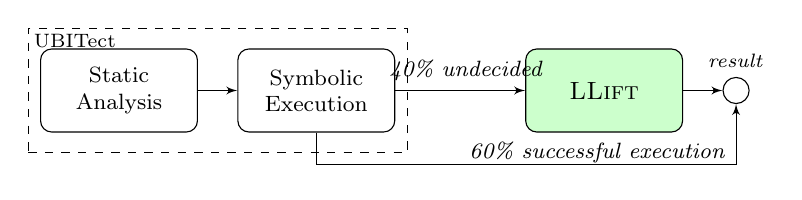
\begin{tikzpicture}[
    block/.style={rectangle, draw, text width=5em, text centered, rounded corners, minimum height=3em},
    line/.style={draw, -latex'},
    node distance=0.3cm and 0.5cm
]

% UBITect
\node[block, font = \footnotesize] (static) {Static Analysis};
\node[block, font = \footnotesize, right=of static] (symbolic) {Symbolic Execution};


\path[line] (static.east) -- (symbolic.west);
% \path[line] (symbolic.east)  |- ++(0.7cm, 0)  -| (final.north) node[midway, above] {};

% Your approach
% \node[block, fill = orange!20, below=1.2cm of static] (preprocess) {Preprocess};
\node[block, fill = green!20, right=1.65cm of symbolic, font = \small] (chatgpt) {\work};

\node[circle, draw,  right= of chatgpt, text centered, minimum height=0.1pt, label=\textit{\scriptsize result}] (final) {};
% \node [block, above=of final, font=tiny]{\textit{final result}};

\path[line] (symbolic.east) -- (chatgpt.west) node [pos =0.55, sloped, above, font=\footnotesize] {\textit{40\% undecided}};
\path[line] (chatgpt.east) -- (final.west);

% Boxes
\node[dashed,  draw, fit={(static) (symbolic)}, inner sep=0.15cm, minimum height=4.5em] (ubitect_box) {};

% \begin{scope}[on background layer]
% \node[dashed, draw, fill=gray!15, fit={(preprocess) (chatgpt) }, inner sep=0.15cm, minimum height=4.5em] (our_box) {};
% \end{scope}


\node[anchor=north west, inner sep=2pt, font=\scriptsize] at (ubitect_box.north west) {UBITect};
% \node[anchor=north west, inner sep=2pt, font=\tiny] at (our_box.north west) {CodeHitch};

% Data flow
\path[line] (symbolic.south) |- ++(0,-0.4cm) -| (final.south) node[pos=0.6, above, left=0, font=\footnotesize] {\textit{60\% successful execution}};

\end{tikzpicture}
 
  }
  \caption{The overview of \work. Start with the discarded cases by UBITect
   and determine whether these potential bugs are true or false.
   % \zhiyun{change the figure to filter style}
   }
  \label{fig:design-flow}
  \vspace{-5pt}
\end{figure}


\begin{figure}[t]
\hspace{-15pt}
\includegraphics[width=.5\textwidth]{figures/minted/case_problem.pdf}
\caption{A typical type of potential UBI bug. For each suspicious variable \(X\), we expect it to 1) have an initializer function that probably initializes  \(X\) and 2) use \(X\).  
}
\label{fig:prob_scope}
\end{figure}


\section{Problem Formulation}
\label{sec:problem}

\subsection{Definitions and Scope}


\subsubsection{Use-Before-Initialization.} A \acf{UBI} bug refers to the erroneous scenario where a variable \( v \) is accessed or involved in any operation prior to its correct initialization. 
% \yizhuo{"any operation" is not consistent with the definition in UBITect, may need extra explanation later in the evaluation.}
% Assumes \(d(v)\) is the declaration of \(v\), \( u(v) \) is a  use operation of \( v \), and \(i(v)\) initializes \(v\).
Let:

\begin{itemize}
\item 
\(d(v)\) represent the declaration of \(v\).
\item 
\(u(v)\) signify a use operation involving \(v\).
\item 
\(i(v)\) denote the initialization operation of \(v\).
\end{itemize}

if there exists \(d(v)\) and \(u(v)\), then \(v\) is \textit{used before initialization} if:
% \yu{why $\exists v$?}
\begin{equation}
% \nexists i(v) : d(v) < i(v) < u(v)
\exists v : (d(v) < u(v)) \land \neg (\exists i(v) : d(v) < i(v) < u(v))
% \yizhuo{...\neg (\forall i(v) : d(v) < i(v) < u(v))?}
\label{eq:ubi_def}
\end{equation}
where \( < \) indicates a temporal sequence in the program execution. 
% The important characteristic of UBI is that it requires a \textit{use} of a possibly uninitialized variable, which gives us a foundation for our optimization.


\cut{
\subsubsection{\acf{SAR}.} 
A \acf{SAR} of UBI bug is a tuple defined as:
\begin{equation}
\text{SAR} = \langle v, F \rangle
\end{equation}
Where:
\begin{itemize}
    \item \(v\) refers to the uninitialized variable being accessed.
     \item \(F\) specifies the function or context housing the variable \(v\) and its usage \(u(v)\). 
    % \zhiyun{do we mean the function that defines the variable? we should make it clear that we consider only local variables}
\end{itemize}

\cut{
\subsubsection{System Definition} Let \work denote a framework defined as:
\begin{equation}
\work : \text{SAR} \times \text{LLMs} \rightarrow \text{Bug Detection}
\end{equation}
where \work interfaces with SAR and LLMs (e.g., ChatGPT) to systematically identify and reason about UBI bugs from the reports generated by static analysis tools.

The \work is designed to be compatible with bug reports generated by various static analysis tools. In the scope of this paper, our primary focus lies on UBI in C programming languages. To that end, we have chosen UBItect, a state-of-the-art tool specifically developed for detecting UBI bugs.
}

\subsubsection{Framework Definition.}
We define \work as a framework that processes Static Analysis Reports (SAR) to detect bugs:

\begin{equation}
\work(\text{SAR}) \rightarrow \text{Bug Detection}
\end{equation}

Here, \work takes a SAR as input and outputs a bug analysis result. While in principle generalizable to other types of static analysis tools, the prototype of our framework is primarily aligned with UBI detection in the C programming language. 
Specifically, we leverage UBItect which produces the SARs that we want as input to \work.
}

\subsubsection{Postcondition.}

Postconditions encapsulate the expected state or behavior of a system upon the conclusion of a routine~\cite{DBLP:books/ph/Meyer97}. Specifically, they detail the guarantees a routine offers based on its observable outcomes.

For a routine \( R \), consider its set of outcomes as
\(\mathcal{O}\). These outcomes are defined as \textit{updates} to its parameters (and return value) for a path of \(R\). Particularly, \(\mathcal{O}\) does not include
initialization for variables for convenience.
In the study of UBI bug, for a routine \( R \) that can yield a set of outcomes \( \mathcal{O} \), the postcondition \(\mathcal{P}\)
can be defined as:
\begin{equation}
\mathcal{P}_R: \mathcal{S}(R) \rightarrow  \mathcal{O} \times \texttt{must\_init}
\end{equation}
Here, \(\mathcal{S}(R)\) signifies all possible execution paths through the routine \(R\), 
\(\mathcal{O}\) describes all updates of \(R\) on its variables, and
\texttt{must\_init} is a set of variables that must be initialized. 
% Note that only if a variable ends up with the \texttt{must\_init} outcome will it influence the final bug detection result --- a \texttt{must\_init} variable means that its subsequent uses will not lead to UBI, whereas a \texttt{may\_init} will still lead to a subsequent UBI.



\PP{Motivating Example.}
Consider the \texttt{sscanf()} function in our motivating example. 
Based on these return values, the postconditions assure the initialization of certain variables:

\begin{align*}
    \mathcal{P}(path_1) &: \{{ret \mapsto 0}, \texttt{must\_init} \mapsto \emptyset \} \\
    \mathcal{P}(path_2) &: \{{ret \mapsto 1}, \texttt{must\_init} \mapsto \{a\} \} \\
    \mathcal{P}(path_3) &: \{{ret \mapsto 2}, \texttt{must\_init} \mapsto \{a,b\} \} \\
    \mathcal{P}(path_4) &: \{{ret \mapsto 3}, \texttt{must\_init} \mapsto \{a,b,c\} \} \\
    \mathcal{P}(path_5) &: \{{ret \mapsto 4}, \texttt{must\_init} \mapsto \{a,b,c,d\} \} \\
    \mathcal{P}(path_6) &: \{{ret \mapsto 5}, \texttt{must\_init} \mapsto \{a,b,c,d,n\} \} \\
\end{align*}

\noindent
Here, the \(path_1 - path_6\) represent different possible paths in the \texttt{sscanf()} and
each path corresponds with a different postcondition.


For UBI detection, not every associated postcondition is relevant; instead, only the outcomes making the \(u(v)\) reachable are \textit{critical}. The constraints of the use are  \textit{\textbf{post-constraints}} \( \mathcal{C}_{post} \) \cite{path_program_analysis}. The \textit{qualified postcondition}, \( \mathcal{P}_{qual} \), is a subset of \( \mathcal{P} \) refined by \( \mathcal{C}_{post} \):

\[
\mathcal{P}_{qual} = \mathcal{P} |_{\mathcal{C}_{post}}
\]

For the \texttt{sscanf()} case, if the post-constraint is \( \mathcal{C}_{post} = \text{ret} \ge 4 \), the qualified postcondition would be \(\mathcal{P}(path_5) \wedge \mathcal{P}({path_6})\), which ensures that variables \texttt{a, b, c,} and \texttt{d} must be initialized; therefore, all variables used subsequently are initialized, and no UBI happens.

In subsequent discussions, unless otherwise specified, the term \textit{`postcondition'} shall denote \textit{`qualified postcondition'}.


\subsection{Post-Constraint Guided Path Analysis}
\label{subsec:postcondi_work}


When analyzing a routine or function in a path-sensitive manner, the number of paths to explore can grow rapidly. Fortunately, if we have information about what the function is expected to achieve (given by \(\mathcal{C}_{post}\)), we can prune paths that inherently don't meet those expectations. We categorize
two scenarios, \textbf{\textit{direct application}} and \textbf{\textit{outcome conflicts}}, in applying this optimization.
 % these scenarios into:

% \begin{enumerate}
%     \item \textbf{Direct Application}: The \(\mathcal{C}_{post}\) can be directly applied as a path constraint. Paths that inherently contradict this applied constraint can be discarded.
%     \item \textbf{Outcome Conflicts}: Some paths within the function might produce outcomes that contradict the \(\mathcal{C}_{post}\). If such conflicts are detected, these paths can be pruned.
% \end{enumerate}



Let \( R \) be the routine or function under analysis and \( \mathcal{S}(R) \) be its path set. Let \( path \in \mathcal{S}(R) \) refer to a specific path in \( R \). Besides, Each path \(path\) has an associated path constraint \(p\) that dictates its feasibility. These two optimizations can be formed with:

% \begin{enumerate}

\PP{Direct Application.} For direct application, the post-constraint \(\mathcal{C}_{post}\) can be directly applied as a path constraint. 
A \textit{path} can be discarded if:

\begin{equation*}
\neg ( p(path) \land \mathcal{C}_{post}) 
\end{equation*}

This implies that if a \( path \) inherently contradicts the post-constraint, it can be removed from consideration.

\PP{Outcome Conflicts.} Let \( \mathcal{O}(p) \) denote the set of all outcomes or effects produced by path \( p \). A \textit{path} can be pruned if any of its outcomes conflict with the post-constraint:

\[
 \exists o \in \mathcal{O}(path) : \neg (o \land \mathcal{C}_{post})
\]

 This stipulates that if an outcome from \( path \) inherently contradicts the post-constraint, that path can be disregarded in the analysis.

% \end{enumerate}

\PP{Correctness.} The validity of these optimization methods can be proved by contradiction. Consider an instance where one of these paths is executed. If this path conflicts with the $\mathcal{C}_{\text{post}}$, it would render $u(v)$ unreachable. Thus, it becomes evident that such paths can be pruned without sacrificing the correctness of the analysis.

We provide a concrete example of how we perform these optimizations in \S\ref{subsubsec:postcon_rule}.


% With postcondition awareness analysis, the exploration space of paths in
% the function can be effectively reduced and therefore makes the path-sensitive analysis feasible.



% \begin{figure}[t]
% \begin{minted}[xleftmargin=10pt, linenos, fontsize=\footnotesize, escapeinside=@@]{c}
% int caller_function(){
%     int X; // declare of suspicious variable @\(X\)@ 
%     ...
%     ret = init(&X); // initializer of @\(X\)@ 
%     ...
%     if (ret == SOME_CONDI) // a check for postconditition [not required]
%         use(X); // use of @\(X\)@ 
% }
% \end{minted}
% \caption{A typical case of potential UBI bug. For each suspicious variable \(X\), we expect it to 1) have an initializer function that probably initializes  \(X\) and 2) use \(X\). Usually, it includes a check 
% for the
% }
% \label{fig:prob_scope}
% \end{figure}

\cut{
\subsection{Assumptions}
\haonan{need to revise}
Let \(V\) be a variable, \(F\) be a function, and \(C\) be a callee function.

\begin{enumerate}
    \item \(A_1\): We restrict our analysis to patterns where \(V\) is declared in \(F\) and is passed to \(C\) for initialization.
    \item \(A_2\): Initialization of \(V\) in \(C\) can occur with multiple layers of indirection.
    \item \(A_3\): Direct initializations of \(V\) in \(F\) are excluded from the scope.
\end{enumerate}
}



% These patterns are visualized in Figure \ref{fig:}.
\subsection{Conceptual Workflow}
\label{subsec:concept_wf}

Given a bug report containing a suspicious variable \( v \) and its residing function \( F \), the workflow \( \Phi \) is as follows:

\begin{enumerate}
    \item \( \Phi_1(F, v) \rightarrow \{i(v)\} \): Identify potential initializers for \( v \) from the bug report.
    \item \( \Phi_2(F, i(v)) \rightarrow \mathcal{C}_{post} \): Extract the \( \mathcal{C}_{post} \) from the bug report for each \(i(v)\).
    \item \( \Phi_3(F, \{i(v), \mathcal{C}_{post} \}) \rightarrow \text{InitStatus}(v) \): Summarize the initialization status for variable \( v \) after all possible initializers completion (merge multiple initializers). 
    % with respect to their corresponding \( \mathcal{C}_{post} \).
\end{enumerate}


% Figure \ref{fig:wf-case} also illustrates the conceptual workflow with three steps. 
% \yu{do we explain the figure? If not, explain it here}


\noindent
\textbf{Decision Policy.}
% \label{subsec:decicison_policy}
The decision policy \(\Delta\) is defined as: 
% \haonan{actually we also support multiple inits}
\begin{align*}
    \Delta(\text{InitStatus}(v) = \textit{must\_init}) & : \text{non-bug} \\
    \Delta(\text{InitStatus}(v) \neq \textit{must\_init}) & : \text{potential bug}
\end{align*}



% In this policy, we simply consider all non-\textit{must\_init }(or, \textit{may\_init}) to be potential bugs. This may produce false 
% alarms, as UBITect may falsely report non-use variable \(v\)\yu{what do you mean here by mentioning UBITect}. Besides, since we only consider \(F\) and
% ignore \(F\)'s call stack (\eg \(F\)'s caller) and other global memories,
% our method may lack path constraints and only over-approximates the initialization status, which can also result in false positives.
% \yu{A better explain here is to show this policy would keep the sound and would not introduce FN. Then mention a little about possible FP. We should try to  show the benefits of what we do.}

In this policy, we adopt a conservative approach by treating all variables not explicitly marked as \textit{must\_init} as potential vulnerabilities.
% We aim to minimize the introduction of false negatives and maintain soundness to the greatest extent possible. This is one contributing factor to the low occurrence of false negatives in our approach, should they exist. 
And it is worth noting that this policy may introduce some false positives. For example, it might \textit{over-approximate} preconditions.
% \yu{How about this.}



Conceptually, \work will not miss more bugs. The post-constraint guided path optimizations and decision policies are safe.



\subsection{Turns and Conversations in LLMs}
\label{subsec:turn_convo}

% \yu{must we have this sub section?}

We define two key concepts in interacting with LLMs: \textit{turn} and \textit{conversation}.

\squishlist
    \item \textbf{Turn:} A turn encapsulates a singular interaction with the LLM. Formally, it's defined as a tuple, $(p, r)$, where $p$ represents the problem or question, 
    % which in our context might be a code snippet or a query related to postcondition, 
    and $r$ denotes the LLM's response.

    \item \textbf{Conversation:} Leveraging the capabilities of LLMs often necessitates a series of interactions, especially for complex problem-solving. A conversation is an ordered sequence of turns. A conversation comprising $n$ turns can be expressed as $[(p_1, r_1), (p_2, r_2), \ldots , (p_n, r_n)]$.
\squishend


\section{Design} 
\label{sec:design}
% \zhiyun{High-Order Consideration? Does this section summarize all considerations or only a subset (most critical?)}

% \yu{more reasons but not just what we do}

% \haonan{I understand the "design consideration" means there are multiple design choices and we pick one and give reasons. Therefore, there're all considerations: 1) LLM vs. static analysis; 2) Muli-step design}

In Section \S\ref{subsec:concept_wf}, we introduced a conceptual workflow. Elaborating on that foundation, Figure~\ref{fig:wf-case} showcases a compelling illustration of our methodological approach. Yet, translating this workflow into practice presents its challenges. 
% Despite harnessing the robust knowledge and reasoning prowess of leading-edge LLMs, 
Even with the advanced knowledge and analytical capabilities of cutting-edge LLMs,
achieving optimal results remains a challenge. Throughout the development of \work, we identified several obstacles and subsequently introduced four distinct design components to effectively address these challenges.





\begin{figure}
    \hspace{-25pt}
    \includegraphics[width=.51\textwidth]{figures/workflow_case.drawio.pdf}
\caption{Example run of \work. For each potential bug, \work \  \libcirc{1} (\(\Phi_{1}\)) identifies its initializer, 
    \libcirc{2} (\(\Phi_{2}\)) extracts the post-constraints of the initializer, and
     \libcirc{3} (\(\Phi_{3}\)) analyzes the behavior of the initializer with the post-constraints via LLM. }
     \label{fig:wf-case}
\end{figure}







\subsection{Design Challenges}
\label{sec:design_chall}

It is non-trivial to prompt LLMs effectively~\cite{zhao2023survey, prompt_engineering}. We meet the following challenges and propose solutions correspondingly in designing \work.



\squishlist
\item \textbf{C1. Limited Understanding of Post-constraint.} 
% Unlike static analysis and symbolic execution, 
Despite LLMs (\eg GPT-4) are able to comprehend the definition of post-constraint and apply them in simple scenarios, we found their capacity to utilize this knowledge in actual program analysis—such as summarizing function behavior in line with specific post-constraint —to be limited. This critical limitation often results in unpredictable and inconsistent outcomes.
%This is because extracting postconditions requires an intricate combination, filtering, and even solving multiple path constraints, which is complicated.



\item \textbf{C2. Token Limitations.} It is known that \acp{LLM} have token limitations. For example, GPT-3.5 supports 16k tokens and GPT-4 supports 32k 
tokens \cite{openai_2023_function}. This means that we do not want to copy a large number of function bodies in our prompts to LLMs.




\item \textbf{C3. Unreliable and Inconsistent Response. }
% \zhiyun{include hallucination?}} 
LLMs are known to result in unreliable and inconsistent responses due to
\textit{hallucination} and \textit{stochasticity} \cite{zhao2023survey}.
Stochasticity refers to the inherent unpredictability in the model's outputs \cite{vaswani_attention_2017}; and the hallucination refers to LLMs generating nonsensical or unfaithful responses \cite{ji_survey_2023, zheng_why_2023}.
By design, the stochasticity can be mitigated with lower \textit{temperature}, a hyperparameter controlling the degree of randomness in outputs~\cite{salamone_what_temp_2021}; however, 
 reducing temperature may impair the model's exploring ability  \cite{xu_systematic_2022} and therefore 
 may miss \text{corner} cases that result in vulnerabilities.



\squishend





\begin{figure}
  \centering
  \includegraphics[width=0.48\textwidth]{figures/wf-v3.drawio.pdf}
  % \scalebox{0.9}{
  %   \hspace{-5pt}
  %   \input{figures/wf-v.tex}
  % }
  \caption{The workflow of \work. Given a potential bug, we let LLM first identify the initializer and then extract its post-constraints (Convo.1),  
  then leverage them to summarize the behavior of the initializer (Convo.2).
   A conversation consists of prompts (boxes) and responses (edges).} 
  \label{fig:wf}
  % \vspace{-10pt}
\end{figure}


\subsection{Design Overview}

We will discuss our design strategies to address the above challenges in the rest of the section. Before that, we provide a high-level overview of our solution.

\squishlist
\item To tackle challenge \textbf{C1} (Post-constraint), we propose to encode \textbf{\textit{(D\#1) Post-Constraint Guided Path Analysis}} by teaching LLMs with examples, or \textit{few-shot in-context learning}, of post-constraints.
This approach enables LLMs to learn from a small number of demonstrative examples, assimilate the underlying patterns, and apply this understanding to process post-constraint guidance in our analysis. 

\item  To tackle challenge \textbf{C2} (Token Limitation), We employ two strategies: 
 \textbf{\textit{(D\#2) Progressive Prompt}.} 
Instead of copying a large number of function bodies (\ie subroutines), we only provide function details on demand, \ie when LLMs are not able to conduct a result immediately.
 \textbf{\textit{(D\#3) Task Decomposition.}} We break down the problem into sub-problems that can be solved in independent conversations, \ie \textit{a sequence of prompt and response pairs}. 
% Note that the token limit is reset for each independent conversation.

\item To tackle challenge \textbf{C3} (Unreliable Response), we employ the following strategies: 
\textbf{\textit{(D\#4) Self-Validation.}} We ask LLMs to review and correct their previous responses. This helps improve the consistency and accuracy based on our observation. 
Besides, \textit{\textbf{(D\#2) Progressive Prompt}} and \textit{\textbf{(D\#3) Task Decomposition}} also help to deal with this challenge. Additionally, we implement \textit{\textbf{majority voting}} by running each case multiple times and use majority voting to combat stochasticity. 
\squishend



We elaborate the design of (D\#1 - \#4) \textit{\textbf{Post Constraint Guided Path Analysis}}, \textbf{\textit{Progressive Prompts}}, 
\textbf{\textit{Task Decomposition}}, and
\textbf{\textit{Self-Validation}} detailed in the rest of this section.
The effectiveness and efficiency of these design strategies are rigorously evaluated in \S\ref{sec:comparison}, revealing a substantial enhancement in bug detection within the Linux kernel.


\subsection{Design \#1: Post-Constraint Guided Path Analysis}
\label{subsec:postcondi}

The Linux kernel frequently employs return value checks as illustrated in Table \ref{tab:postcondi_types}. Through our detailed examination of non-bug instances, we found that 
a path-sensitivity analysis can effectively eliminate over 70\% of these negative cases. However, path-sensitive static analysis usually suffers from path explosion, especially in large-scale codebases like the Linux kernel.

Fortunately, we can prompt the LLM to collect \(\mathcal{C}_{post}\) and summarize the function with respective to the 
\(\mathcal{C}_{post}\). It is worth noting that current LLMs (\eg GPT-4) are not natively sensitive to the sensitivity; without any additional instructions, LLMs usually overlook the post-constraints.
Therefore, we teach the LLM to be sensitive to post-constraints rules through few-shots in-context learning. We describe the design details as follows:



\begin{table}

\caption{Two types of post-constraints and their variants.}
\label{tab:postcondi_types}
\vspace{-3pt}
\includegraphics[width=.48\textwidth]{figures/minted/case_few_shot.pdf}
% \vspace{-8pt}
\end{table}

\subsubsection{Post-Constraints Extraction.} 
To extract the \textit{qualified postcondition}, we first determine the post-constraints that lead to the use of suspicious variables.
We incorporate few-shot in-context learning to teach LLMs how to extract such constraints from the caller context. Table \ref{tab:postcondi_types} demonstrates how we teach LLM with in-context learning. We focus primarily on two types of code patterns:
% \yu{why those two?}

\squishlist
\item \textbf{Check Before Use.} 
% Type A exemplifies this pattern: for the use of \texttt{a,b,c,d} to be reached, it must first satisfy the check \texttt{sscanf(...)>=4}. 
Type A is our motivating example; by looking at its check, the post-constraint should be \(ret \ge 4\).
Type A' describes a similar case with \texttt{switch-cases}, with expected output \(ret \mapsto \texttt{crticial\_case}\).
% \yu{Type A of post-constraints should be more clear.}
%\zhiyun{Have we defined this term? I don't understand what it means.}
\item \textbf{Failure Check.} This pattern captures the opposite of the first pattern. They commonly occur in the Linux kernel where the error conditions cause the use to become unreachable, as illustrated in Type B, the post-constraint is \(err \mapsto 0\).
Type B' depicts a variant where the initializer keeps retrying til success, and therefore with expected output \(ret \mapsto 0\), which indicates
its first successful execution to break the endless loop.
% Teaching LLMs the variants helps them differentiate subtle differences.
%Here the checks are performed without early returns (\ie without \texttt{break/return/goto} to prevent reaching the usage). In Type B', any sub-scenarios of
%the postcondition can reach \texttt{use(a)}; therefore, we mark it \texttt{null}.
\squishend


\subsubsection{Function Behavior Summarization.} 
%Postconditions serve a vital role in weeding out irrelevant paths when summarizing the initializer. 
Once we obtain the \textit{post-contraints} in Convo.1, we feed them to the LLM to obtain the behavior summary in Convo.2 . For example, we provide the following: 

% \vspace{-3pt}
\begin{lstlisting}[numbers=none]
{
 "initializer": "ret = sscanf(str,'%u.%u.%u.%u%n',&a,&b,&c,&d,&n)",
 "suspicious": ["a", "b", "c", "d"],
 "postconstraint": "ret >= 4"
}
\end{lstlisting}
% [breaklines, fontsize=\footnotesize, baselinestretch=0.8]{json}

% \end{minted}
% \vspace{-5pt}

The LLM may respond with 

% \vspace{-5pt}
\begin{lstlisting}[numbers=none]
{
 "ret": "success",
 "response": {
   "must_init": ["a", "b", "c", "d"],
   "may_init": [{"name":"n", "condition": "ret > 4"}]
  }
}
\end{lstlisting}

\cut{
We can see that the response encodes the postcondition concisely
where \texttt{a,b,c,d} are considered \texttt{must\_init} and \texttt{n}
is considered \texttt{may\_init} because it is initialized only when \(ret > 4\), and not when \(ret \mapsto 4\).
}

The response succinctly encapsulates the function behavior, where variables \texttt{a,b,c,d} are classified as \texttt{must\_init}, and \texttt{n} is categorized as \texttt{may\_init}. This is due to the initialization of \texttt{n} only occurring when \(ret > 4\), and not when \(ret \mapsto 4\).

Note that this seemingly simple interaction with LLMs can be challenging for static analysis or symbolic execution. Consider the \texttt{sscanf()} example, even if the analysis is aware that the qualified postcondition should be limited to those where \(ret \ge 4\),
it would still need to enumerate the paths inside of \texttt{sscanf()}, which involves loops and can easily lead to timeouts as explained in \S\ref{sec:ubitect}.



\subsubsection{Apply Path Analysis}
\label{subsubsec:postcon_rule}

% \cut{
Following \S\ref{subsec:postcondi_work}, Figure \ref{fig:postcondi_use} presents a concert example of post-constraint guided path analysis. This case shows a simple initializer \(i(a)\) of the variable \(a\). Given an early return, the initialization in line 4 may not be executed. As such, the \textit{qualified postconditions} become contingent on the \textit{post-constraints} \(\mathcal{C}_{post}\). There are:

\squishlist
\item If the use of variable \texttt{a} is unconditional, \ie \(\mathcal{C}_{post}=\top\).
% the relevant path constraints would be empty (\ie \texttt{constraints: null}). 
In this case, the variable \(a\) is labeled as \texttt{may\_init} given that the initialization \textit{may not} be reached.

In general, if all path constraints and outcomes of \texttt{must\_init} are \textit{disjoint from} \(\mathcal{C}_{post}\),
no path can be pruned out. We could also conclude \(a\) as \textit{may\_init}.
\item If the use of variable \(a\) is conditional with constraints, \ie \(\mathcal{C}_{post}\neq\top\), two cases emerge:
\begin{enumerate}
\item \(\mathcal{C}_{post}\) clashes with the constraints of the path (e.g., \texttt{some\_condi}), or
\item \(\mathcal{C}_{post}\) conflicts with the path outcome (e.g., \texttt{return -1}).
\end{enumerate}
In these instances, \(\mathcal{C}_{post}\) could be \texttt{some\_condi} or \texttt{func(...)==0} and we can designate \texttt{*a} as \texttt{must\_init}. 
\squishend



\cut{
\vspace{3pt}
\noindent
While there are a few other cases we have not considered for postconditions throughout the Linux kernel, the above rules cover most of the scenarios we have encountered. We highlight some interesting examples in \S\ref{subsec:excuse}. It's worth noting that the few-shots in-context learning methodology is extensible, making it easy to incorporate new rules and scenarios.
}









\begin{figure}
\begin{minipage}{.15\textwidth}
\centering
\begin{lstlisting}[language=c]
int func(int* a){  
  if(some_condi)
    return -1;
  *a = ... // init 
  return 0;
}
\end{lstlisting} 
\end{minipage}%
\begin{minipage}{.35\textwidth}
\centering
\vspace{-8pt}
\begin{tabular}{p{4.5cm}}

\text{\small \(\texttt{must\_init} =\emptyset\)  if:} \\
% \texttt{\small\{postconstraint: null\}} \\
\text{\small \(\mathcal{C}_{post} = \top \)} or  \\
% \text{\small\(\forall ps \in p(\mathcal{S}): ps \perp \mathcal{C}_{post}\ \wedge
% \forall o \in \mathcal{O}: o \perp \mathcal{C}_{post}\) } \\
\text{\small\(\forall ps \in \{ \neg \texttt{some\_condi} \}: ps \perp \mathcal{C}_{post}\ \wedge \)} \\
\hspace{15pt}\text{\small \(\forall o \in \{ret \mapsto 0\}: o \perp \mathcal{C}_{post}\) } \\
% \text{\small\(\forall p \in \{ \texttt{some\_condi}, \neg \texttt{some\_condi} \}: p \perp \mathcal{C}_{post}\)} \\
\hline
\text{\small  \(\texttt{must\_init} =\{a\}\)  if:} \\
% \texttt{\small\{postcondi: !some\_condi\}} or\\  
\text{\small \( (\neg \texttt{some\_condi}) \wedge \mathcal{C}_{post} \) or} \\
% \texttt{\small\{postcondi: func(...) == 0\}} \\
\text{\small\( (ret \mapsto 0) \wedge \mathcal{C}_{post} \) }\\
\end{tabular}


\end{minipage}


\caption{A sample case of initializer \texttt{func}, \texttt{*a} is \texttt{may\_init} or \texttt{must\_init} under different post-constraints. }
\label{fig:postcondi_use}
\end{figure}




\subsection{Design \#2: Progressive Prompt}
\label{subsec:iter_prompt}

\cut{
In the Linux kernel, it is common for each function to call many other functions further. Therefore, for the initializer summarizing task, if we do not provide
any further function definitions and ask LLMs to deliver a response instantly, they might fail due to a lack of knowledge.
However, if we put every relevant function definition at once, it will quickly exceed the limitation of context windows of LLMs.

To solve this dilemma, we propose to provide function definitions \textit{what LLMs need} selectively. As demonstrated in Figure \ref{fig:wf}, 
when LLMs analyze the initializer, the \textit{Progressive Prompt} design
fosters an ongoing interaction with the LLMs instead of soliciting an immediate response.
In this progressive exchange, 
we always prompt LLMs with: ``\textit{If you experience uncertainty due to insufficient function definitions, please indicate, and I will provide them}''. Upon receiving a request for additional information from LLM, we animatedly extract the necessary information from the source code and provide them to LLMs, enabling them to reevaluate and generate an improved response.
This back-and-forth interaction continues until the LLM garners sufficient information to deduce the initializer's behavior or until we exhaust the available information. If we cannot provide further information, for example, we can not find the requested function in the Linux source; we prompt it to continue analysis conservatively.
} 

The Linux kernel has an extremely large codebase. Summarizing an initializer using LLMs without providing any supplementary function definitions can result in incomplete or erroneous responses. On the other hand, flooding the LLM with every relevant function definition upfront risks exceeding their context window limitations.

To address this dilemma, we choose to progressively provide function definitions as needed. 
Illustrated in Figure \ref{fig:wf}, this approach, which we refer to as \textit{Progressive Prompt}, fosters a dynamic interaction with the LLM rather than expecting a response in one shot.
Throughout this iterative exchange, we consistently prompt the LLM: \textit{``If you encounter uncertainty due to a lack of function definitions, please signal your need, and I'll supply them''}. 
Should the LLM need more information, \work will promptly extract the relevant details on demand from the source code and provide it to the LLM \textit{automatically}, enabling it to reassess and generate a more accurate response. 
% \yizhuo{highlight the autmation here?}

% \haonan{how to prompt it stably}
Specifically, We teach the LLM to ask for more information with a specific format:
\begin{lstlisting}[numbers=none]
    [{"type":"function_def", "name":"some_func" }]
\end{lstlisting}

Subsequently, \work scans this format in the LLM's response. For each requested function definition,
\work supplies its corresponding code along with comments extracted from the Linux source code.
Though GPT-4 may seek other types of information beyond function definitions (\eg struct definitions), we currently limit our support to requests pertaining to function definitions.
% \yu{reason?}

The iterative process continues until either the LLM no longer requests additional information, or \work cannot supply the requested details. In certain situations where \work is unable to provide more information (\eg the definition of an indirect call), \work will still prompt the LLM to proceed with the analysis. In these instances, the LLM is encouraged to infer the behavior based on the available data and its inherent knowledge, thereby facilitating continued analysis even when not all information is directly accessible.

\cut{
Note that our current design has a simple strategy to handle indirect calls. First, \work simply asks the LLM to identify the indirect call target, which can succeed in certain cases as shown in the evaluation. If the LLM fails to identify the target, we will simply force it to generate a summary of postconditions based on its knowledge of the Linux kernel, without the definition of any indirect call target.
\zhiyun{added a new paragraph.}
}

%In situations where we cannot provide further data --- for instance, if the requested function cannot be located in the Linux source \zhiyun{how would this happen? limitations of our implementation?} --- we encourage the LLM to continue its analysis with a conservative approach.


\cut{
A key advantage of this progressive design lies in its efficiency. Rather than cluttering the conversation with all potential functions, we only provide those pertinent to the ongoing analysis. This approach considerably reduces the use of tokens, making the process more streamlined and resource-efficient. By fostering iterative, targeted exchanges, the progressive prompt design helps leverage the LLM's capabilities more effectively while maintaining focus on the analysis at hand.
}

% Interavive promp

% The function summary produced by ChatGPT is intentionally \textit{\textbf{different}} from the one generated by UBITect. In UBITect, the function summary is calculated solely through the analysis of a function and its callees, without considering the context in which the caller invokes the function. As a result, it is correct  for a UBITect function summary to indicate that a specific parameter \textit{``may not''} be initialized, given that a path exists in the function where initialization does not occur.
% In contrast, \work takes into account the calling context, including concrete arguments and return value checks, when analyzing a function. These elements serve as additional constraints that can influence the function's behavior. By providing this context when invoking a function, \work is better equipped to determine if a parameter will be initialized.






\subsection{Design \#3: Task Decomposition}
\label{subsec:multi-step}

We systematically apply the principle of task decomposition, a vital element of our design process. This concept is incorporated primarily in two distinct ways.

\vspace{3pt}
\noindent
\textbf{Multistage Problem Solving.} 
\cut{
First, as Figure \ref{fig:wf} outlined, 
\work employs two separate \textit{conversations} to finish the task. Each conversation (\ie independent sessions) contains
several turns of \textit{prompts and responses}. \work first
extracts the initializer and its \textit{post-constraints} (subtasks 1 and 2) in Convo.1, 
and then summarizes the postconditions (subtask 3) based on the \textit{post-constraints} in Convo.2. 
Without task decomposition, we will combine all three subtasks into a single conversation, and prompt it to finish all three subtasks at once.
We also evaluate this option in \S\ref{subsec:expr_comp}.
}
% Firstly, task decomposition is evident in the way we structure our work. 
As illustrated in Figure \ref{fig:wf}, we employ a two-conversation approach to complete the task. Each conversation, essentially consists of multiple iterations of prompts and responses. The first conversation (Convo.1) is dedicated to extracting the initializer and its associated post-constraints (subtasks 1 and 2), while the second conversation (Convo.2) focuses on summarizing the function (subtask 3) based on the previously identified post-constraints. This division allows a more manageable and effective way of achieving the task, compared to combining all three subtasks into a single conversation. The efficacy of this task decomposition approach is further evaluated in \S\ref{subsec:expr_comp}.


\vspace{3pt}
\noindent
\textbf{Thinking in English.} 
Our workflow necessitates a structured output, such as a JSON format, for automation. However, we observe that LLMs often produce suboptimal results when directly prompted to output in this format. As LLMs build responses incrementally, word-by-word, based on preceding outputs \cite{vaswani_attention_2017}, direct prompts to output JSON may interrupt their thought progression. This emphasizes the importance of initially soliciting responses in natural language to ensure comprehensive and effective reasoning. Consequently, we instruct the LLM to first articulate their thought processes in English, followed by a subsequent prompt to transform their response into a JSON summary.


%From our preliminary test, %the zero-step design can hardly identify buggy code, and the one-step design is significantly worse than the multi-step design, which are consistent with recent literature reports \cite{ma_scope_2023, tian_is_2023}.
% \haonan{can we also cite our own paper?}.




\subsection{Design \#4: Self-Validation}
\label{subsec:self_refine}

\cut{
LLMs sometimes exhibit erratic or inconsistent behaviors, especially in complex scenarios that involve intricate logic. For example, for a initializer 
with postcondition \texttt{must\_init} if \(ret \mapsto 0\), the LLM 
sometimes might ignore the post-constraint and believe it is
\texttt{may\_init} even with the exact 
post-constraint \(ret \mapsto 0\).
On the other hand, LLM might pretend 
non-exist post-constraint and mistakenly conclude
a \texttt{may\_init} case to \texttt{must\_init}.
Namely, LLMs brings both false positives and false negatives in detecting bugs.
}

At times, LLMs can display unpredictable or inconsistent behaviors, particularly in complex scenarios involving detailed logical constructs. Consider a case where an initializer carries the postcondition \texttt{must\_init} if \(ret \mapsto 0\). LLMs may still mistakenly assume it to be \texttt{may\_init}, despite the explicit presence of the post-constraint \(ret \mapsto 0\).

Conversely, an LLM might erroneously interpret a non-existent post-constraint and incorrectly infer a \texttt{may\_init} case as \texttt{must\_init}. 
This phenomenon is known as \textit{hallucination}.
Essentially, the hallucination can lead to both false positives and false negatives in bug detection, thereby affecting accuracy and reliability. 



In addition to task decomposition,  we also introduce the concept of \textit{self-validation} to enhance reliability.
Before the LLM reaches its final conclusion,
this method reinforces specific rules, allowing the LLM to reassess their previous responses for adherence and make necessary corrections. We observed that this practice yields better results. We evaluate the effect of self-validation in \S\ref{sec:comparison}.
% \haonan{actually it seems now, it 1) increases the consistency (but we don't have a data?) 
% 2) improve the recall, instead of precision}

% \textbf{In Postcondition Extraction.} 
As seen in Figure \ref{fig:wf}, we employ self-validation in both conversations. 
By prompting a list of  \textit{correct} properties that we expect, LLMs can verify and correct their results by themselves automatically.
% We specifically request LLMs to follow two crucial rules when performing self-validation: 1) Postconditions should not include any suspicious variables. 
% 2) A postcondition must directly influence the reachability of the use of the suspicious variable. Therefore, in the case of error checks, without an explicit \texttt{return/break/goto} command rendering subsequent usage impossible, it should not be a valid postcondition.
%\zhiyun{needs editing after postcondition definition is finalized.}

\cut{
% \textbf{In Initializer Summary.} 
When summarizing initializers, we observe a propensity of the LLM to reach a `safe', yet imprecise choice (\ie \texttt{may\_init}) without self-validation. 
Thus, we incorporate self-validation to encourage the LLM to reassess \texttt{may\_init} and \texttt{must\_init} cases to heighten precision. This strategy is also woven into our progressive prompt design. If the LLM requests more information to complete the analysis, we revert to the progressive prompting stage and sustain the interaction. This synergy between self-validation and progressive prompts leads to a more robust analysis and a more productive engagement with the LLM.
}
% we eval
% \yizhuo{Good to add the prompts.}\yizhuo{The goal of self-validation is to reduce the false positives, and we need to make this clear and describe why the precision benefits from this refinement.}
% It is interesting that we do not combine the self-validation with the JSON generation step. The combination can improve speed and reduce cost; however, it only works well with some simple rules. If we want LLM to review its last result and correct itself, separation is necessary.

% self-validation need to be designed very carefully as it is actually a double-edged sword. It can improve the precision of LLM mostly, but it can also make the result worse sometimes. We need to keep the consistency with previous prompts to 


% \begin{figure}
% \begin{minted}[xleftmargin=10pt, breaklines, linenos, fontsize=\footnotesize]{c}
% struct assoc_array_edit *assoc_array_insert(...){
%   ...
%   switch (assoc_array_walk(... &result)) {
%   case assoc_array_walk_tree_empty:
%     return ...
%   case assoc_array_walk_found_terminal_node:
%     if (!assoc_array_insert_into_terminal_node(... &result))
%     ...
%   }
% }
% \end{minted}
%     \caption{\haonan{Derived from \texttt{lib/assoc\_array.c}. suspicious variable \texttt{result}, used in Line 7}}
%     \label{fig:my_label}
% \end{figure}



% \subsection{initialization function identify and postcondition collects}

% Given the initial context and the suspicious variable (that being used), we ask
% ChatGPT which function could potentially initialize the variable. This process could be done via a simple string match; say, if this variable being passed as
% parameter or a comprehensive def-use analysis. However, a perfect analyzer 
% working in Linux may require significant efforts to embed much knowledge such as concurrency and callback functions.  
% To make our life easier,
% we directly ask ChatGPT for this specific task. 

% With the initialization function, we then prompt ChatGPT to collect all postconditions. We only care that condition that could be expressed in relationship of return values of initialization function.
% In our tests, most of the cases are perfectly handled by ChatGPT except for a few examples of variable reuse. A light-wight static analyzer could convert 
% the code to the form of SSA and solve this issue.









% \vspace{3pt}
% \noindent\textbf{Prompt Design.}
\subsection{Additional Prompting Strategies}
\label{subsec:other_prompt}

In order to further optimize the efficacy of our model, we have incorporated several additional strategies into our prompt design:

\squishlist

\item \textbf{Chain-of-Thought.}
Leveraging the Chain-of-Thought (CoT) approach, we encourage the LLMs to engage in stepwise reasoning, using the phrase \textit{``think step by step''}. This not only helps generate longer, comprehensive responses, but it also provides intermediate results at each juncture of the thought process. Previous studies suggest the CoT approach considerably enhances the LLMs' reasoning capabilities~\cite{chen_when_2023}. We incorporate the CoT strategy into every prompt.

\item \textbf{Source Code Analysis.}
Rather than analyzing abstract representations, we opt to focus our attention directly on the functions within the source code. This approach not only economizes on token use compared to LLVM IR, but also allows the model to leverage the semantic richness of variable names and other programming constructs to conduct a more nuanced analysis.

%\item \textbf{Reasoning in Natural Language.}
%We consistently instruct the LLMs to articulate their thought processes in English, ultimately synthesizing their findings into a JSON summary at the end of the conversation. As LLMs such as GPT construct responses word-by-word, based on preceding outputs, direct prompts to generate JSON can disrupt their reasoning process. The process of thinking aloud in natural language is thus crucial to facilitate thorough and effective reasoning.

\squishend

% \item \textbf{Prioritize Rules and Eliminate Conflicts.} \haonan{it is also important to keep different rules not conflicted...}








\cut{
There are many interesting details in building effective prompts.
For example, prompting LLM output with \textit{conditions} of each \texttt{may\_init} (\ie in what cases it will initialize) improves its performance. Moreover, sometimes replace a word by its synonym can impact the results. 
For example, if we tell LLM with \textit{`don't do something'} --
it sometimes understands exactly the opposite -- \textit{`do something'}.
Considering they do not affect the overall approach, interested readers can discover these details from our open-sourced detailed prompts implementation and experiments.
}


\cut{
\vspace{3pt}
\noindent
Designing effective prompts involves mastering many intriguing nuances. For instance, enhancing the LLM's output by specifying the \textit{conditions} under which each \texttt{may\_init} (i.e., conditions in which initialization will occur) can boost its performance. 
Furthermore, equally impactful can be the strategic substitution of words with their synonyms. A striking example is the paradoxical interpretation of negations by the LLM. If prompted with a command like \textit{`don't do something'}, the LLM occasionally comprehends it as \textit{`do something'}, the exact reverse of the intended instruction. 
% \zhiyun{so what is our solution for this do something example?} \zhiyun{I suggest we remove the paragraph altogether as it seems confusing.}
\haonan{I personally like it, but can also remove}
}

\vspace{3pt}
\noindent
% While these subtle factors don't alter the overarching strategy, they do enrich its execution and can be pivotal in optimizing performance.
There are still some interesting details in designing an effective prompt
but due to space constraints and without changing the overall strategy, we will not list them all. Readers intrigued can delve into the intricacies of our open-sourced prompt\footnote{\href{https://sites.google.com/view/llift-open/prompt}{https://sites.google.com/view/llift-open/prompt}} design and experimental implementations to gain a deeper understanding.
% \zhiyun{align the prompt language in all detailed conversations. mention demo fully automated.}
% \zhiyun{need to decide whether we want to provide an end-to-end example for the submission.} \haonan{why not, we can put them later; I also need do for our short paper}



















\cut{
% \noindent
In a perfect world, an ideal static analysis tool can alternatively perform these steps, too. However, implementing an efficient static analysis is challenging due to the fundamental challenges of static
analysis, as we mentioned in \S\ref{subsec:funda_chall}.
Instead, LLM provides a simple integration that makes this workflow possible, especially for these 
potential bugs that UBITect cannot verify due to time or memory out, as Figure \ref{fig:design-flow} demonstrates.
}
% The LLM conducts these three steps.
% Each stage will be discussed in more detail in the following sections.
% We discuss each component of the workflow in the following sections.
% We elaborate on these techniques in the following sections: progressive prompt in \S\ref{subsec:iter_prompt}, self-validation in \S\ref{subsec:self_refine}, few-shots learning of postcondition  in \S\ref{subsec:postcondi}, and the rest in \S\ref{subsec:other_prompt}.


\cut{
\noindent
\textbf{LLM vs. Static Analysis.} 
Given the significant challenges of static analysis as highlighted in \S\ref{subsec:funda_chall}, LLM-based approaches  emerge as a flexible and powerful alternative. In an ideal world, a perfect static analysis tool would provide precise and correct answers for these steps.
% possess the ability to analyze all possible program execution paths and provide precise and comprehensive answers regarding various program properties, including program correctness.} 
% \yu{it is called Parametric Static Analysis}
However, the reality is often starkly different, as implementing an efficient and universally applicable static analysis tool is complex, time-consuming, and fraught with inherent limitations.

LLMs, on the other hand, present an innovative avenue to circumvent these challenges. They offer a simple, efficient integration that makes advanced analysis workflows viable, particularly for potential bugs that tools like UBITect struggle to verify due to resource constraints. As depicted in Figure \ref{fig:design-flow}, \work can effectively take these inconclusive cases and find hidden bugs in them.
% LLMs can facilitate an efficient and effective bug verification process,
}






\cut{
\subsection{Design Exploration}
\label{design_explo}
\zhiyun{consider moving to design section}


% Before our final three-stage design (referenced as \textit{multi-step}), we initially explored more straightforward design possibilities. 
It is not trivial to apply the LLM. 
% Notably, we contemplated employing LLM to directly determine whether a code carries UBI bugs (\textit{zero-step}), or specifying the target function and original context first and then directing it to generate a summary (\textit{one-step}).
First, prompting LLM to directly judge each potential bug (referred to \textit{zero-step}) is unreliable.
Second, even taking our workflow, expecting that LLM can give a direct answer in a single conversation (referred to \textit{one-step}) is not a good idea.  We describe these two explorations as follows.

\subsubsection{Zero-step Design}


We initially experimented with the zero-step design methodology. In this process, we provided an in-depth definition of a UBI bug, followed by a direct copy of the caller context, pinpointing the suspicious variable that might be used before initialization. We adhered to the guidelines mentioned in \S\ref{sec:design}, such as Chain-of-Thought and progressive prompting.

We validated this methodology on several case studies. One was a false positive (\ie not a bug) case (\texttt{cpuid}), while the other was an actual bug (\texttt{p9pdu\_readf}). Despite our efforts, GPT-4, the most potent LLM, fell short in both instances. 
% Intriguingly, we observed that even when explicitly encouraged to ask follow-up questions about function definitions, GPT-4 would instead generate a seemingly plausible but incorrect answer without seeking additional information.

Recent research, such as \cite{tian_is_2023}, indicates that ChatGPT struggles with accurately explaining the intentions of incorrect code. This also shows current LLM does not diliver a reliable summariaztion from the code directly.
% However, this should not lead to the assumption that LLM cannot provide meaningful interpretations of programming languages. Our two subsequent design strategies serve to demonstrate this.



\subsubsection{One-step Design}
The one-step design employs our workflow. Specifically, we prompt LLM to summarize a function call whether it \texttt{may\_init} or \texttt{must\_init} the suspicious variable. Therefore, for a potential UBI bug, if there is an initializer that \texttt{must\_init} the suspicous bug, we can conclude there's not a real bug.

While the one-step design surpasses the zero-step, it can still overlook real bugs. As illustrated in Figure \ref{fig:p9_read}, \texttt{p9pdu\_readf} is a case in point. Upon examination of the function \texttt{p9pdu\_vreadf}, GPT-4 occasionally assumes that the \texttt{pdu\_read(...)} in Line 10 - functioning as a protective check - must succeed, thereby leading to the initialization of its parameter at Line 14.
 

While the one-step design surpasses the zero-step, it can still overlook real bugs. In the one-step design, we prompt GPT-4 to pay close attention to the \textbf{\textit{postconditions}} of the initializer. However, it often confuses the postcondition in the initial caller context with subsequent checks. This observation laid the groundwork for our multi-step design, which involves the separate extraction of postconditions in advance, providing explicit constraints and prompting for analysis.
}

% \cut{
% \begin{figure}
% \begin{minted}[xleftmargin=10pt, linenos, breaklines, escapeinside=||, fontsize=\footnotesize]{c}
% int p9_check_zc_errors(...){
%   err = p9pdu_readf(..., "d", &ecode);
%   err = -ecode;
% }
% // similar to `sscanf/vsscanf`, p9pdu_readf is a wrapper of p9pdu_vreadf with va_args
% int p9pdu_vreadf(... const char *fmt, va_list ap){
%    switch (*fmt) {
%      case 'd':{
%        int32_t *val = va_arg(ap, int32_t *);
%        if (pdu_read(...)) {
%        	errcode = -EFAULT;
%        	break;
%        }
%        val = ...;  // initialization
%   }
%   return errcode;
% }
% \end{minted}
%     \caption{Code snippet of \texttt{p9pdu\_readf} and its usecase, derived from \texttt{net/9p} 
%     }
%     \label{fig:p9_read}
% \end{figure}
% }

% \subsubsection{Multi-step Design}

 % The multi-step design
 % first only extracts the initializer and its call context: the postconditions. And then performs the analysis. 
 % Theoretically, this task could be done with a relatively straightforward intraprocedural dependence
 %  analysis. However, due to the varieties of Linux code, adaptation to the Linux kernel is non-trivial. For simplicity, we chose to implement it using LLM and the experiment
 %  shows it performs well in most situations.
\section{Implementation}
% \haonan{In this section, we describe the prototype of \work.}

We implement the prototype of \work based on OpenAI's API~\cite{openai_2022_introducing_2022}
(\ie gpt-4-0613).
% with GPT-4 with 8k tokens. GPT-4 is the most powerful LLM so far; we use it to demonstrate all potential of \work.
% Specifically, under version gpt-4-0613 with a token limit of 8,192.
% All implementation is finished by the end of
% July 2023.
% \yu{Evaluation?}
We describe some implementation details in the following aspects:


\vspace{3pt}
\noindent
\textbf{Interaction with LLMs.} \work's interaction with LLMs is managed by a simple agent developed in Python, containing roughly 1,000 lines of code. In addition, it uses seven prompts, which altogether constitute about 2,000 tokens in two conversations.
All interactions are \textit{fully automated} via APIs of OpenAI. 
Besides sending prompts and waiting for responses, our agent also 1) interacts with LLMs according to the progressive prompt design, 2) locates function definitions within the Linux source code, and 3) processes responses from LLMs, then receives and stores to a database.

\vspace{3pt}
\noindent
\textbf{Hyper-Parameters.} There are several hyper-parameters in calling the APIs provided by OpenAI. We choose \texttt{max\_token} and \texttt{temperature} to 1,024 and 1.0, respectively. \texttt{max\_token} controls the output length; since LLMs always predict the next words by the previous output, the longer output can benefit and allow its reasoning. However, too many tokens will exhaust the context window quickly, so we pick 1024 as a reasonable balance.

The temperature controls the randomness and also the ability to reason. 
Intuitively, we want the analysis to be as non-random as possible and reduce the temperature (it can take a value between 0 and 2 for GPT models);
however, an overly low temperature can result in repetitive or overly simplistic responses. We set it to 1.0 (also the default of gpt-4-0613), which allows for higher-quality responses, and use strategies such as self-validation and majority voting to improve the consistency of responses.
%balance the need for diverse interpretations without sacrificing the stability and correctness of the analysis.

\cut{
\vspace{3pt}
\noindent
\textbf{Initializer Analysis.} 
% The prototype of \work focuses on providing a high-quality function summary of initializers to assist with UBITect. 
A UBI variable might not have an initializer and be used directly. If used locally, a straightforward intra-procedure analysis can figure it out. Otherwise, if the variable is passed to another function that is not an initializer, the framework of \work can still provide a high-quality summary of use. Considering that, in most cases, the summary of use provided by UBITect is sufficient, we focus on the most critical part that causes inaccuracies, the initializer, in our prototype.
% Our framework can also provide such summaries by design; however, few cases exist. We excluded these cases from our current prototype. In other words, we assume that UBITect is accurate in its summary of parameter usage and that there is no need for \work.
\yu{we should mention what we do in the implementation. not only why}
}





\cut{
\vspace{3pt}
\noindent
\textbf{Majority voting.}
We run each case 3 times and output the majority results (\ie \(\ge\)2 times).
Specifically, we run each case twice to see if any inconstancy and run a third time if any.
}



\cut{
\vspace{3pt}
\noindent
\textbf{Bug decision.} \work produces the use-guided postcondition which effectively classifies the suspicious variable to either \texttt{must\_init}, or \texttt{may\_init}, or \texttt{no\_init}.
We consider \texttt{no\_init} because \zhiyun{add some explanation.}
We employ a simple policy to decide whether the case is a bug: as long as the suspicious variable is classified as \texttt{may\_init} or \texttt{no\_init},
we consider it a bug.

}


\cut{
\vspace{3pt}
\noindent
\textbf{Self-validation.} 
Implementing self-validation in our design presents intriguing aspects with implications for the performance of LLMs. One might consider combining self-validation with the JSON generation step to expedite the process and reduce computational costs. However, this approach is only effective for simpler rules. For scenarios that demand the LLM to reassess its previous output and make adjustments, separating the self-validation process is critical.

self-validation, while mostly beneficial in enhancing the precision of LLMs, needs meticulous design and execution, as it can be a double-edged sword. At times, it can inadvertently detract from the accuracy of the result. Therefore, maintaining consistency with previous prompts and carefully examining the scope and context of self-validation is essential to leverage its benefits without compromising the overall outcome. The balance between precision enhancement and result stability is the key to unlocking the full potential of self-validation in LLM-based static analysis.
}


% \textbf{Variable Alias.} \haonan{Similar to the last one ....}

% \textbf{Incorrect Initializer Extract.} The identifying of initializer and the collecting postcondition might fail, despite
% rarely. Most of the failures are due to the suspicious variable
% does not exist in the initial context.



% Analyzing these cases requires a combination of the possibilities of all operations on these variables.

% \subsection{Prompt Implementation}

% Limited by space, we put the detailed prompts with several real conversations on an anonymous page\footnote{\href{https://anonymous.4open.science/r/LLIFT-B2B5/conversation.md}{https://anonymous.4open.science/r/LLIFT-B2B5/conversation.md}}.

% \textbf{}
% \subsubsection{Initializer \& Postcondition Extraction.} The conversation for initializer and postcondition extraction is relatively simple.
% As Figure \ref{fig:wf} depicted before, we use the few-shots in-context learning to teach LLM how to extract postconditions. Additionally, 
% we incorporate some clarifications for confused cases, such as multiple postconditions, and then let LLM itself refine its response.


% \subsubsection{Initializer Behavior Summary.}

% \work covers the following substances in prompts:
% \begin{itemize}
% % \item[\ding{118}] Analyze function calls to assess parameter initialization.
% \item[\ding{118}] Incorporate function return value checks in the analysis.
% \item[\ding{118}] Ensure field-sensitive analysis, focusing on parameter fields.
% \item[\ding{118}] Request additional information (e.g., function
% definitions) if needed.
% \item[\ding{118}] Classify parameters/fields as \texttt{must\_init} or \texttt{may\_init} based
% on initialization conditions.
% \item[\ding{118}] Present analysis results in JSON format for easy integration.
% \end{itemize}

% For the return value check, we have demonstrated how it can benefit 
% the motivating example in Figure~\ref{fig:sscanf}, \ie \texttt{sscanf(...)>=4}.


% Limited by space, We present detailed prompt with several complete conversations with GPT-4 on an anonymous page\footnote{\href{https://anonymous.4open.science/r/LLift-Open/Cases/README.md}{https://anonymous.4open.science/r/LLift-Open/Cases/README.md}}.
%we will demonstrate all conversations containing our experiments after the paper gets accepted.
%\haonan{finish the end-to-end conversation}
% Although adding the prompt with more detailed explanations or examples (\ie few-shot) might be
% viable, we opted for this differentiation to enable potential future use. \zhiyun{I don't really follow the last sentence.}


\begin{table*}[]
    \centering
    % \caption{Found Use-Before-Initialization (TP) From Time/Memory out Cases \haonan{rename...} \zhiyun{should mention the kernel version otherwise the line number is useless.}}
    \caption{True bugs identified by \work from Random-1000, analyzing in Linux v4.14}
    \label{tab:table_rq1}
\scalebox{0.9}{
\begin{tabular}{llllll}
\toprule
\textbf{Initializer}               & \textbf{Caller}                            & \textbf{File Path }                                      & \textbf{Variable}          & \textbf{Line} \\
\midrule
read\_reg                & get\_signal\_parameters              & drivers/media/dvb-frontends/stv0910.c      & tmp                & 504                                 \\
regmap\_read             & isc\_update\_profile                 & drivers/media/platform/atmel/atmel-isc.c   & sr                 & 664                                 \\
ep0\_read\_setup         & ep0\_handle\_setup                   & drivers/usb/mtu3/mtu3\_gadget\_ep0.c       & setup.bRequestType & 637                                 \\
regmap\_read             & mdio\_sc\_cfg\_reg\_write            & drivers/net/ethernet/hisilicon/hns\_mdio.c & reg\_value         & 169                                 \\
bcm3510\_do\_hab\_cmd    & bcm3510\_check\_firmware\_version    & drivers/media/dvb-frontends/bcm3510.c      & ver.demod\_version & 666                                 \\
readCapabilityRid        & airo\_get\_range                     & drivers/net/wireless/cisco/airo.c          & cap\_rid.softCap   & 6936                                \\
e1e\_rphy                & \_\_e1000\_resume                    & drivers/net/ethernet/intel/e1000e/netdev.c & phy\_data          & 6580                                \\
pci\_read\_config\_dword & adm8211\_probe                       & drivers/net/wireless/admtek/adm8211.c      & reg                & 1814                                \\
lan78xx\_read\_reg       & lan78xx\_write\_raw\_otp             & drivers/net/usb/lan78xx.c                  & buf                & 873                                 \\
t1\_tpi\_read            & my3126\_phy\_reset                   & drivers/net/ethernet/chelsio/cxgb/my3126.c & val                & 193                                 \\
pci\_read\_config\_dword & quirk\_intel\_purley\_xeon\_ras\_cap & arch/x86/kernel/quirks.c                   & capid0             & 562                                 \\
ata\_timing\_compute     & opti82c46x\_set\_piomode             & drivers/ata/pata\_legacy.c                 & \&tp               & 564                                 \\
pt\_completion           & pt\_req\_sense                       & drivers/block/paride/pt.c                  & buf                & 368                                \\
\bottomrule
\end{tabular}
}

\end{table*}

\section{Evaluation}
\label{sec:eval}

Our evaluation aims to address the following research questions.

% \begin{itemize}
\squishlist
\item \textbf{RQ1 (Precision):} How accurately is \work able to identify bugs?
\item \textbf{RQ2 (Recall):} Is there a possibility for \work to miss real bugs?
\item \textbf{RQ3 (Comparison):} How does the performance of individual components within \work compare to that of the final design?
\item \textbf{RQ4 (Model Versatility):} How does \work perform when applied to LLMs other than GPT-4?
% How do our design principles contribute to the performance of \work?
% Compared to other design approaches and LLMs, how superior is \work?
% How does \work perform compared to other design approaches and different LLMs?
\squishend

% \end{itemize}
\vspace{3pt}
\noindent

We evaluate RQ1 to RQ3 in GPT-4, under API from OpenAI with version gpt4-0613.
For RQ4, we also test GPT-3.5 with version gpt-3.5-turbo-0613 and Claude 2 additionally for comparison.
% Claude 2 was run manually on its webpage.



\subsection{Dataset}
% The data incorporated in our research was harvested from the output generated by UBITect. To be specified, all the considered cases were derived from UBITect's positive static analysis results that resulted in either a timeout or exhaustion of memory during the symbolic execution. 
% % These situations imply an inconclusive verdict from UBITect on the respective cases, which could potentially contribute to false negatives or overlooked flaws in the system. This is where the utilization of \work presents an alternative avenue to investigate these cases.

% The static analysis of UBITect produces 140k positives, and symbolic execution can only handle 60\% of them and left 
% 53k cases. Due to the capacity limit of OpenAI (\$600 per month when we do the experiment), 
% we cannot run all of them 
% before our submission.

Our experiment data, sourced from UBITect, includes all potential bugs labeled by its static analysis stage but experienced timeout or memory exhaustion during its symbolic execution stage. 
Overall, UBITect's static analysis stage produced 140,000 potential bugs, with symbolic execution able to process only 60\%, leaving 53,000 cases unattended, which means that these cases are generally difficult for static analysis or symbolic execution to decide
We craft the following dataset from 53,000 cases to evaluate \work:



~\noindent(1) \textbf{Random-1000.} We randomly chose 1,000 from the 53,000 cases for testing. However, there are 182 cases where there are no initializers, which are automatically recognized and filtered (see \S\ref{sec:problem}). The remaining 818 cases are used in evaluating precision, \ie the ratio of true positives to false positives. 

~\noindent(2) \textbf{Bug-50.} This dataset comprises the 52 confirmed UBI bugs previously identified by UBITect. It is used as ground truth for assessing recall by verifying if any true bugs were overlooked.

~\noindent(3) \textbf{Cmp-40.} This dataset comprises 27 negative and 13 positive cases selected from the Random-1000. We utilize this dataset to illustrate which of our design strategies contributed most to the outcome of our solution.
% \yu{still random selected? We should mention it. And why 27 and 13?}



% \subsection{Basic Statistics}
% Execution time is not our focus. \zhiyun{This is a bad phrase to use. I would just remove it.}
\PP{Turns and Conversations.}
Due to the progressive prompt, each case may require different turns (pairs of a prompt and a response). In Random-1000, the average number of turns is 2.78, with a max of 8 and a variance of 1.20. 

% \PP{Time.}
% Due to the progressive prompt, the execution time of each case varies. In Random-1000, the average number of turns (\ie pairs of a prompt and a response) is 2.78, with a max of 8 and a variance of 1.20. 
% Each turn typically takes a few seconds. Note that the exact time for each turn of prompt and response varies depending on the  workload on the OpenAI infrastructure 
% % (sometimes we need to retry due to API failures). 
% Due to the request rate limit of the API, we have to lower the frequency of requests. It takes roughly one day (24 hours) to run through the 1,000 cases. 
% We are unable to do more tests due to the monthly cap.
% \yu{we have explained monthly cap before.}


%\zhiyun{We should translate the number of turns into execution time. Some turns can take longer than others, e.g., depending on how many words there are.}
%\haonan{single executing time is be meaningless, it highly depends on which time you request openai. besides, OpenAI keeps trying to make it more fast}
% \haonan{to reduce RPM, the latency is close to real execution time}


% \zhiyun{If it takes only 24 hours to finish 941 cases, why don't we run more cases? We claim earlier we don't run more because of rate limit. But it doesn't seem to be the true reason?} \haonan{mostly capacity limit, previously only \$600. } \zhiyun{we should state this then.} \haonan{stated before the enumerate}

% \PP{Cost.} GPT-4 currently costs \$0.06 for outputting each 1k tokens. On average, it costs \$0.43 to analyze each potential bug in random-1000. The total budget is \(\sim\)\$430. Therefore, readers may not faithfully reproduce all
% of our experiments if they hate OpenAI (Maybe they love Google and NVIDIA and are happy to spend much more on GPU computation) and refuse to send money to them. Nevertheless, it is feasible to choose samples from our open-source dataset to experiment with.

\PP{Cost.} On average, it costs 7,000 tokens in GPT-4 to analyze each potential bug.
% Also, we spent about 50 human hours inspecting all results and obtain the ground truth.


% \PP{Token Limitation.} \haonan{...} 4 of 


% \PP{Excluded Cases.} 182 cases are excluded due to they are out of our scope as described in Figure \ref{fig:prob_scope} (\ie no initializer function to analyze), and 4 cases exceed the maximum context length while exploring deeper functions in the progressive prompt.

\cut{
\begin{figure}
\begin{minted}[xleftmargin=10pt, linenos, fontsize=\footnotesize]{c}
int ath10k_pci_diag_write_mem(..., int nbytes){
 while (ath10k_ce_completed_recv_next_nolock(..., 
           &completed_nbytes) != 0) {
    mdelay(1);
    if (i++ > DIAG_ACCESS_CE_TIMEOUT_MS) {
      ret = -EBUSY;
      goto done;
    }
  }
  //use of "completed_nbytes"
  ...

}
int ath10k_ce_completed_recv_next_nolock(..., unsigned int *nbytesp){
 ...
 nbytes = __le16_to_cpu(sdesc.nbytes);
 if (nbytes == 0) {
   return -EIO;
 }
 desc->nbytes = 0; 
 /* Return data from completed destination descriptor */
 *nbytesp = nbytes;
   ...
 return 0;
}
\end{minted}
\caption{Code snippet of \texttt{ath10k\_...\_nolock} and its usecase, derived from \texttt{net/wireless/ath/ath10k/ce.c} }
\label{fig:case_while}  
\end{figure}
}

\subsection{RQ1: Precision}
\label{subsec:expr_precision}

% We consider two things for RQ1:

% \begin{enumerate}
%     \item For positive cases, how precise is \work?
%     \item Considering both positive and negative cases, how accurate is \work?
% \end{enumerate}

\work reports 26 positives among the Random-1000 dataset, where half of them are true bugs based on our manual inspection. This represents a precision of 50\%.
% Table \ref{tab:table_rq1} shows the 13 new UBI cases. 
% Interestingly, even though we analyzed the Linux kernel v4.14, which is the version UBITect was capable of supporting, 
In keeping with UBITect and we focus on the analysis of Linux v4.14,  12 of the bugs still exist in the latest Linux kernel.
% We submit the patch of these 13 vulnerabilities to the Linux community.
We are in the process of reporting the 12 bugs to the Linux community.
So far, we have submitted patches for 4 bugs and received confirmation that they are true bugs.
%\zhiyune{with TODO bugs being patched already}. \zhiyun{give a forward reference about case studies.}

% \noindent
% \textbf{Consistency.} LLM is known for its randomness and inconsistency. 

\vspace{3pt}
\noindent
\textbf{Imprecise and Failed Cases.} 
 Despite the effectiveness of \work, there are instances where it does not yield precise results, resulting in 13 false positives by mistakenly classifying \texttt{must\_init} cases as \texttt{may\_init}. Upon a careful examination of these cases, we attribute the imprecision to a variety of factors, which we discuss in detail in \S\ref{subsec:excuse}.
 Briefly, we give a breakdown of them here: \textit{Incomplete constraint extraction} (4 cases), \textit{Information gaps in UBITect} (5 cases), \textit{Variable reuse} (1 case), \textit{Indirect call} (1 case), and \textit{Additional constraints} (1 case). Additionally, there is one false positive caused by inconsistent output (i.e., two false positives in three runs). 
 Four cases exceed the maximum context length while exploring deeper functions in the progressive prompt. %\haonan{failed cases}






\find{
\textbf{Takeaway 1.} \work Can effectively summarize initializer behavior 
and discover new bugs with high precision (50\%).
}


\cut{
\begin{figure}
    \centering
    \includegraphics[width=0.45\textwidth]{figures/con_sr.pdf}
    \caption{self-validation of analyzing case \texttt{axi\_clkgen\_recalc\_rate}, it concludes an incorrect answer
    \texttt{must\_init} at first, and then corrects it to \texttt{may\_init} after the self-validation.}
    \label{fig:con_sr}
\end{figure}
}
  

\subsection{RQ2: Recall Estimate}
\label{subsec:expr_recall}

Conceptually, the core optimization (post-constraint guided path analysis) of \work is sound, 
and we also prompt a series of rules to let LLMs tend to respond ``\texttt{may\_init} when uncertain.
We expect \work would not reject true bugs or with a high recall.

We sample 300 negative cases
from Random-1000 in an effort to see whether we will miss any true bugs. 
We confirm that all are true negatives. Despite the limited data sampled, this result indicates that integrating GPT-4 into our implementation does not introduce apparent unsoundness. 

Further, we test \work on the Bug-50 dataset to see \textit{whether it will miss any bugs discovered by UBITect}.
\work has demonstrated full effectiveness in identifying all real bugs from Bug-50. This result, while encouraging, does not imply that \work is flawless. Detailed data analysis reveals that:
1) There remain some inconsistencies in 3\(\sim\)5 cases
% per run \zhiyun{what is the round? each round consists of 3 runs?} \haonan{per run} \zhiyun{how can a single run experience inconsistencies? it doesn't make sense.} 
occasionally, though they are mitigated by majority voting; and 2) 
all the bugs found by UBITect have trivial post-constraints \((\mathcal{C}_{post}=\top\)) and postcondition of \textit{may\_init} (\(\mathcal{P}_{qual}: \texttt{must\_init} \mapsto \emptyset\)). 
Hence, \work could identify them easily.
It is noteworthy that these cases are already those cases detectable by UBITect. 
Such cases tend to be simpler in nature and can be verified by symbolic execution in UBITect.

% In addition to the Bug-50 dataset, 

% Actually, \(\sim\)40 of Bug-50 cases are unchecked use of \texttt{regmap\_read}.



\cut{
\haonan{3 inconsistent, majority voting can fix}
\vspace{3pt}
\noindent
\textbf{Consistency.} The instability of LLM is well known; however, the results of \work are quite stable. We ran each case in Bug-50 more than three times for each example and obtained consistent outcomes for most cases (48 of 54 are consistent).
}


\cut{
By checking the detailed conversation. We notice our self-validation design contributes to consistency. As Figure \ref{fig:con_sr} demonstrates, when analyzing \text{axi\_clkgen\_recalc\_rate(1)}, it generates an incorrect answer at first by saying \texttt{must\_init}. Such errors are inherently random; fortunately, self-reflection can spot errors in the next dialog and deliver a correct answer at the end.
\zhiyun{This section does not follow the same structure as the previous one. In the previous section, we talk about the incorrect cases first and then explain it is the self-validation that helps with the correct cases the most. Better be consistent.}
\zhiyun{BTW, when I read the evaluation, I still feel the true negative results are useful to mention somewhere. Both RQ1 and RQ2 are about true bugs only.}
}

\cut{
\begin{figure}[t]
  \begin{minted}[xleftmargin=10pt, linenos, fontsize=\footnotesize]{c}
int regmap_read(struct regmap *map, ...)
{
 int ret;
 if (!IS_ALIGNED(reg, map->reg_stride))
 	return -EINVAL;
 map->lock(map->lock_arg);
 ret = _regmap_read(map, reg, val);
 map->unlock(map->lock_arg);
 return ret;
}
\end{minted}
\caption{Definition of \texttt{regmap\_read}, from \texttt{drivers/base/regmap/regmap.c}}
\label{fig:regmap_read}  
\end{figure}
}

\cut{
\vspace{3pt}
\noindent
\textbf{Incorrect Cases.}  The few inconsistencies or incorrectness are caused by missing checks using the \texttt{regmap\_read} function. This is an interesting case,  as shown in Figure \ref{fig:regmap_read};
 this function can fail, e.g., with not aligned registers. Besides, the
further call of \texttt{\_regmap\_read} might either fail or return an error code.
However, failure in reading registers is rare in practice, and therefore it is commonly used in 
Linux kernel directly uses the function without a return value check. Even
 some Linux maintainers don't think they are real bugs (such as \texttt{stm32\_timer\_stop(2)}
 and \texttt{gemini\_clk\_probe}~\cite{boyd_re_2019, cameron_re_2019}. 
 }
 
\cut{
% because according to our definition it should be classified as \texttt{may\_init}, but in reality it is triggered very rarely.
Therefore, GPT-4 sometimes delivers the \texttt{must\_init} result after the self-validation --- based on the knowledge it has trained.
A thorough solution to such problems requires cleaner training data, fine-tuning, or more runs to eliminate the inconstancy. In practice, 
running each case three times and then outputting the results with more occurrences can get the correct results.
}

% \vspace{3pt}
% \noindent
% \textbf{regmap\_read}. 



 % It is not clear to us at this time how GPT-4 is trained to obtain a priori
 % knowledge of whether this function initializes its parameter. If its knowledge
 % comes from extensive ``code feature learning" from well-maintained open source
 % code, then the misclassification of \texttt{regmap\_read} is understandable.



\find{
\textbf{Takeaway 2.} \work has proven effective in identifying UBI bugs, consistently detecting all known instances.
}





\begin{table}[t]
\centering
\caption{Performance evaluation of bug detection tool with progressive addition of design components: Post-Constraint Guided Path Analysis (PCA), Progressive Prompt (PP), Self-Validation (SV), and Task Decomposition (TD). (C) indicates the number of
\textit{C}onsistent cases.}
\scalebox{0.78}{
\begin{tabular}{@{}lcc|cccc@{}}
\toprule
\textbf{Combination} & \textbf{TN(C)} & \textbf{TP(C)} & \textbf{Precision} & \textbf{Recall} & \textbf{Accuracy} & \textbf{F1 Score} \\ \midrule
Simple Prompt & 12(9) & 2(1) & 0.12& 0.15& 0.35& 0.13 \\
PCA & 13(9) & 5(1) & 0.26 &	0.38 & 0.45 &	0.31 \\
PCA+PP & 5(3) & 6(1) & 0.21& 0.46& 0.28& 0.29 \\
% \rowcolor{gray!15}
PCA+PP+SV & 5(2) & 11(8) & 0.33& 0.85& 0.40& 0.48 \\
PCA+PP+TD & 22(14) & 6(4) & 0.55& 0.46& 0.70& 0.50 \\ 
% \hline
% \rowcolor{gray!15}
{PCA+PP+SV+TD} & 25(17) & 13(12) & 0.87& 1.00& 0.95& 0.93 \\ \midrule
\textit{Oracle} & 27(27) & 13(13) & - & - & - & - \\
\bottomrule
\end{tabular}
}
\label{tab:compare}
% \vspace{-10pt}
\end{table}

\cut{
\begin{figure}
    \centering
\begin{minted}[xleftmargin=10pt, linenos, breaklines, escapeinside=@@, fontsize=\footnotesize]{c}
void irlan_close_data_channel(struct irlan_cb *self)
{
  ...
  skb = alloc_skb(IRLAN_MAX_HEADER + IRLAN_CMD_HEADER +
      IRLAN_BYTE_PARAMETER_LEN("DATA_CHAN"),
      GFP_ATOMIC);
  if (!skb)
    return;
  ...

  frame = skb->data;
  ...
}
\end{minted}
    \caption{Code snippet of \texttt{irlan\_close\_data\_channel}, with
    suspicious varaible \texttt{frame(skb->data)}}
    \label{fig:case_frame}
\end{figure}
}

\cut{
\begin{table}[]
\centering
\caption{Abstract of prompt-response behavior in analyzing function \texttt{irlan\_close\_data\_channel} of design combination PCA + PP + SV (\ie without task decomposition).}
\scalebox{0.8}{
\begin{tabular}{p{1.1cm}|p{8.5cm}}
\toprule
\textbf{Prompt} & \textbf{Response} \\ 
\midrule
\textbf{Starting} & The analysis begins with the given function \texttt{alloc\_skb} which calls \texttt{\_\_alloc\_skb}. \texttt{\{ "ret": "need\_more\_info",  "response": [ \{    "type": "function\_def",    "name": "\_\_alloc\_skb" \} ]\}} \\
\hline
\textbf{PP} & Analyzing the \texttt{\_\_alloc\_skb} function, it's seen that \texttt{skb->data} is initialized after successful allocation of \texttt{skb}. If \texttt{skb} is successfully allocated, \texttt{frame} (which is assigned \texttt{skb->data}) is guaranteed to be initialized. \textbf{\textit{Thus, \texttt{frame} should be classified as `must\_init'}}. \\
\hline
\textbf{SV} & 1) The function \texttt{\_\_alloc\_skb} returns \texttt{skb}. If memory allocation fails, \texttt{skb} is \texttt{NULL}. \newline 2) \texttt{skb} is checked after the \texttt{alloc\_skb} call. \textbf{\textit{If \texttt{skb} is \texttt{NULL}, the function returns, leading to a `may\_init' path for \texttt{frame}.}} \newline 3) If \texttt{skb} is not \texttt{NULL}, \texttt{frame} is assigned \texttt{skb->data}, leading to a 'must\_init' path for \texttt{frame}. \newline 4) As both 'may\_init' and 'must\_init' paths exist, \texttt{frame} is considered as 'may\_init' under some conditions, but not all. \\
\bottomrule
\end{tabular}
}
\label{tab:case_frame}
\end{table}
\vspace{-15pt}
}




\subsection{RQ3: Contributions of Design Strategies}
\label{sec:comparison}

In our effort to delineate the contributions of distinct design strategies to the final results, we undertook an evaluative exercise against the Cmp-40 dataset, employing varying configurations of our solution, each entailing a unique combination of our proposed strategies. As illustrated in Table \ref{tab:compare}, the strategies under consideration encompass Post-constraint Analysis (\textit{PCA}), Progressive Prompt (\textit{PP}), Self-Validation (\textit{SV}), and Task Decomposition (\textit{TD}). The findings underscore an overall trend of enhanced performance with the integration of additional design strategies.
% , highlighting their collective impact.
% \yu{should compare PCA+PP+SV+TD with PCA+PP+SV, PCA+PP+TD, PCA+SV+TD, PP+SV+TD.}

% \vspace{3pt}
% \noindent \textbf{Baseline.}
In this study, the \textit{Baseline} corresponds to a straightforward prompt, \textit{"check this code to determine if there are any UBI bugs"}, a strategy that has been found to be rather insufficient for discovering new vulnerabilities, as corroborated by past studies \cite{openai_2023_gpt_4, ma_scope_2023, tian_is_2023}, reflecting a modest recall rate of 0.15 and a precision of 0.12.

% the solution where we simply perform a single prompt, embedding the function definition and the suspicious variable, asking whether there is a UBI bug.
% We can see that its result is clearly the worst.

Incorporating PCA offers a notable enhancement, enabling the LLM to uncover a wider array of vulnerabilities. As shown in Table \ref{tab:compare}, there is a substantial improvement in recall in comparison to the baseline, an anticipated outcome considering PCA's pivotal role in our solution. However, solely relying on this strategy still leaves a lot of room for optimization.
% Adding PP further improves the precision without any negative impact on Recall. 



The influence of Progressive Prompt (\textit{PP}) on the results is quite intriguing. While its impact appears to lower precision initially, the introduction of task decomposition and self-validation in conjunction with PP reveals a substantial boost in performance. Without PP, the LLM is restricted to deducing the function behavior merely based on the function context's semantics without further code analysis. Even though this approach can be effective in a range of situations, it confines the reasoning ability to the information available in its training data. By checking the detailed
conversation, we notice the omission of TD or SV tends to result in the LLM neglecting the post-constraints, subsequently leading to errors.


Beyond influencing precision and recall, Task Decomposition (\textit{TD}) and Self-Validation (\textit{SV}) also play a crucial role in enhancing \textit{consistency}. In this context, a result is deemed \textit{consistent} if the LLM yields the same outcome across its initial two runs. A comparison between our comprehensive final design encompassing all components, and the designs lacking TD and SV, respectively, reveals that both TD and SV notably augment the number of consistent results, and deliver 17 and 23 consistent results in its negative and positive results, respectively, underscoring their importance in ensuring reliable and consistent outcomes.
% \zhiyun{if we have time, consider improving the consistency a bit further.}


Finally, TD also holds significance in terms of conserving tokens. 
% During our evaluation, we observed two instances in the PCA+PP and PCA+PP+SV configurations where the token limitations of GPT-4 were exceeded. 
In our evaluation phase, we identified two instances within the PCA+PP and PCA+PP+SV configurations where the token count surpassed the limitations set by GPT-4. However, this constraint was not breached in any case when TD was incorporated. 
%This reduction in token usage enables our solution to manage a more diverse array of functions in the Linux kernel, significantly expanding its practicality and usefulness.


\find{
\textbf{Takeaway 3.} All of \work's design strategies contributed to the positive results. 
}



\begin{table}[]
    \centering
    \caption{Comparison of different LLMs on real bugs, from a subset of Bug-50}
\scalebox{1.0}{
\begin{tabular}{lccccc}
\toprule
\multirow{2}{*}{\textbf{Caller}}            & \multicolumn{2}{c}{\textbf{GPT}} & \multirow{2}{*}{\textbf{Claude2}}    & \multirow{2}{*}{\textbf{Bard}}   \\
                                    &   \textbf{4}  & \textbf{3.5} &  &  \\
% \textbf{Caller} & \textbf{GPT-4} & \textbf{PAC}  & \textbf{GPT-3.5} & \textbf{Claude2} & \textbf{Bard } \\
\midrule
  % \rowcolor{gray!40}
  % \multicolumn{4}{l}{\textit{\textbf{False Negatives of UBITect}}} \\ 
%\text{pv\_eoi\_get\_pending}       &  \ding{51} &  \ding{51} &  \ding{51}             \\
%\text{p9\_check\_errors}           &  \ding{51} &  \ding{51} &  \ding{51}             \\
  % \rowcolor{gray!40}
  % \multicolumn{4}{l}{\textit{\textbf{True Positives of UBITect}}} \\ 
\text{hpet\_msi\_resume}           &  \ding{51} &  \ding{51} &  \ding{51}  &  \ding{55}          \\
\text{ctrl\_cx2341x\_getv4lflags}  &  \ding{51} &  \ding{51} &  \ding{55}  &  \ding{55}          \\
\text{axi\_clkgen\_recalc\_rate}   &  \ding{51} &  \ding{51} &  \ding{51}  &  \ding{51}          \\
\text{max8907\_regulator\_probe}   &  \ding{51} &  \ding{51} &  \ding{51}  &  \ding{51}          \\
\text{ov5693\_detect}              &  \ding{51} &  \ding{51} &  \ding{55}  &  \ding{51}          \\
\text{iommu\_unmap\_page}          &  \ding{51} &  \ding{55} &  \ding{51}  &  \ding{55}          \\
\text{mt9m114\_detect}             &  \ding{51} &  \ding{51} &  \ding{51}  &  \ding{51}          \\
\text{ec\_read\_u8}                &  \ding{51} &  \ding{51} &  \ding{51}  &  \ding{51}          \\
\text{compress\_sliced\_buf}       &  \ding{51} &  \ding{51} &  \ding{55}  &  \ding{51}          \\
\bottomrule
\end{tabular}
}

\label{tab:res_cmp}
\end{table}


\subsection{RQ4: Alternative Models}
\label{subsec:expr_comp}

% \haonan{explain gpt-3.5}


Table \ref{tab:res_cmp} provides a comprehensive view of the performance of our solution, \work, when implemented across an array of LLMs including GPT-4.0, GPT-3.5, Claude 2 \cite{anthropic_2023_claude}, and Bard \cite{krawczyk_bards_2023}. GPT-4 passes all tests, while GPT-3.5, Claude 2, and Bard exhibit recall rates of 89\%, 67\%, and 67\%, respectively. Despite the unparalleled performance of GPT-4, the other LLMs still produce substantial and competitive results, thereby indicating the wide applicability of our approaches.

It is imperative to note that not all design strategies in our toolbox are universally applicable across all language models. Bard and GPT-3.5, in particular, exhibit limited adaptability towards the progressive prompt and task decomposition strategies. Bard's interaction patterns suggest a preference for immediate response generation, leveraging its internal knowledge base rather than requesting additional function definitions, thereby hindering the effectiveness of the progressive prompt approach. Similarly, when task decomposition is implemented, these models often misinterpret or inaccurately collect post-constraints, subsequently compromising the results. To harness their maximum potential, we only apply the PCA design specifically (\ie without other design strategies) for GPT-3.5 and Bard.
% \yizhuo{Modify to we applied the PCA to them as that's the only thing we can do.}
% \zhiyun{this paragraph can be made more clear. We did not say (1) with more design strategies, they perform even worse, and (2) why would the results be better with fewer strategies. Let me explain with a concrete confusion of mine: to me, with and without progressive prompt, it should not change the results much for GPT-3.5 and Bard. This is because anyway they will ignore the progressive prompt direction -- basically acting the same as if there is no progressive prompt.}
% \haonan{My guess is when we put too many things, GPT-3.5 pays less attention to the rules in our starting prompt (or, simply because GPT-3.5 suffers more survive hallucination); Bard directly ignores PP, so there is no effect.
% I don't explain it because these phenomena are not easy to describe}

Contrasting the GPT series, Bard and Claude 2 demonstrate less familiarity with the Linux kernel and are more prone to failures due to their unawareness of the \texttt{may\_init} possibility of initializers.

%we will show later in \S\ref{subsec:case_study}, \texttt{get\_user\_pages\_unlocked}. Claude 2 guesses according to the function and parameter name and 
%does not recognize its purpose. Bard gives a plausible but incorrect response.



\find{
\textbf{Takeaway 4.} 
GPT-4 remains at the pinnacle of performance for \work, yet other LLMs can achieve promising results. 
}

% \subsection{RQ4: Comparing to symbolic execution}


\begin{figure}
\hspace{-15pt}
\includegraphics{figures/minted/case_sgl_map.pdf}
    \caption{Case Study I (Loop and Index). Derived from \texttt{drivers/scsi/st.c} 
    }
    \label{fig:sgl_pages}
\end{figure}






\subsection{Case Study}
\label{subsec:case_study}
In this case study, we pick three interesting cases demonstrating the effectiveness of \work in analyzing function behaviors and detecting uninitialized variables. 
All these cases are undecided for the previous static analyzer, UBITect.
We put the complete conversations on an anonymous online page for reference\footnote{\href{https://sites.google.com/view/llift-open/case-studies}{https://sites.google.com/view/llift-open/case-studies}}.
% \zhiyun{Think about whether we want to do this, given the extra alignment we need.}


% \haonan{show more subtle cases, to impresee people how smart (much benefit of its knowledge) it is }


% \zhiyun{alias analysis automatically performed by ChatGPT.}

% LLM, especially for GPT-4, even shows its ability in non-trivial program analysis.

% \vspace{3pt}
% \noindent
% \textbf{Alias Analysis.} For different function call; and pointer assign

% \vspace{3pt}
% \noindent
% \textbf{Context Sensitivity and Path Sensitivity.}

\vspace{3pt}
\noindent
\textbf{Loop and Index.} Figure \ref{fig:sgl_pages} presents an intriguing case involving the variable \texttt{pages[j]}, which is reported by UBITect as used in Line 17 potentially without being initialized. Unfortunately, this case is a false positive which is hard to prune due to loops. Specifically, the initializer function \texttt{get\_user\_pages\_unlocked()}, which is responsible for mapping user space pages into the kernel space, initializes the \texttt{pages} array allocated in Line 3. If \texttt{get\_user\_pages\_unlocked()} is successfully executed, \texttt{pages[0]} through \texttt{pages[res-1]} pointers will be initialized to point to struct page instances. 
% \zhiyun{should emphasize this case is difficult for UBITect (timeout?)} 
% \haonan{done}
%\zhiyun{should mention \texttt{res} being the return value.}
%\haonan{should we show it in more detailed?}

To summarize the behavior, \ie \texttt{must\_init} facts under conditions where the use is reachable,
we must first extract the \textit{post-constraints} that lead to the use of \texttt{pages}. Through interacting with ChatGPT, \work successfully extracts it:
% \zhiyun{TODO: Haonan will copy the JSON result here.}
\begin{lstlisting}[numbers=none]
{
    "initializer": "res = get_user_pages_unlocked(uaddr, nr_pages, pages, rw == READ ? FOLL_WRITE : 0)",
    "suspicious": ["pages[j]"],
    "postconstraint": "res < nr_pages && res > 0 && j < res",
}
\end{lstlisting}

After feeding the post-constraints to LLM, \work then successfully obtains the result:
% \zhiyun{TODO: Haonan will copy the JSON result here}

\begin{lstlisting}[numbers=none]
{
    "ret": "success",
    "response": {
        "must_init": ["pages[j]"],
        "may_init": [],
    }
}
\end{lstlisting}

As we can see, GPT-4 exhibits impressive comprehension of this complex function. 
It perceives the variable \texttt{pages[j]} being used in a loop that iterates from \texttt{0} to \texttt{res-1}. This insight leads GPT-4 to correctly deduce that all elements in the \texttt{pages} array must be initialized, \ie they are \texttt{must\_init}. This example underscores GPT-4's proficiency in handling loop and even index sensitivity.

\begin{figure}
\hspace{-15pt}
\includegraphics{figures/minted/case_hv_pci.pdf}
    \caption{Case Study II (Concurrency and Indirect Call). Derived from \texttt{drivers/pci/host/pci-hyperv.c}
    }
    \label{fig:hv_pci}
\end{figure}



\vspace{3pt}
\noindent
\textbf{Concurrency and Callback.} Consider the case illustrated in Figure \ref{fig:hv_pci}. At first glance, UBITect flags Line 10 for potentially using the variable \texttt{comp\_pkt.completion\_status} before initialization. The function's body seemingly lacks any code that initializes it, leading UBITect to report it as a potential bug.  However, the mystery unravels when we examine \texttt{hv\_pci\_generic\_compl()}, the actual initializer function assigned to \texttt{pkt} in Line 4. The variable in question is indeed initialized, but intriguingly, its initializer emerges from a concurrent function instead of within its own thread. Here \texttt{wait\_for\_completion()} is a synchronization primitive that pauses the current thread and waits for the new thread (\ie \texttt{hv\_pci\_generic\_compl()}) to complete.
Despite this complexity, GPT-4 adeptly navigates the concurrency and callback handling, pinpointing the accurate initializer and outputting a precise result.

It is worth noting that we do not encode any knowledge about the Linux kernel synchronization primitives. 
\work prompts LLMs with  \textit{``The `initializer' must be the `actual' function that initializes the variable.''}
and then LLMs can automatically identify the function \texttt{hv\_pci\_generic\_compl()}
% by copying the entire function body of \texttt{hv\_pci\_enter\_d0}, it 
as the initializer of \texttt{comp\_pkt.completion\_status}.

% \and asking it to identify
% the initializer. Below is a core part of the prompt: 
% \zhiyun{TODO: Haonan will provide an example.}

% \zhiyun{consider adding another case study of inline assembly.}
\vspace{3pt}
\noindent
\textbf{Unfamiliar Function.} 
As previously delineated in \S\ref{subsec:cap}, LLMs possess the inherent ability to recognize the semantics (\eg postconditions) of common functions like \texttt{sscanf()}. However, some argue that \textit{``the LLM simply learns everything from the internet and acts merely as a search engine''} \cite{chiang_chatgpt_2023}. This viewpoint is challenged by the case illustrated in Figure \ref{fig:p9_read}.

The case presents an intriguing real-world bug. The function \texttt{p9pdu\_readf()} mirrors \texttt{sscanf()} in structure, yet lacks a check of its return value, leaving the parameter \texttt{ecode} at risk of being uninitialized, i.e., if \texttt{pdu\_read()} returns non-zero in line 19 (thus ``break'' early).
Notably, unlike \texttt{sscanf()}, where GPT-4 can provide a precise summary of the function without asking for its definition,
it does request the function definition of \texttt{p9pdu\_readf()}, as it is not as ubiquitous as \texttt{sscanf()}.  

Furthermore, our solution not only produces the correct outcome for this particular case but also pinpoints that \texttt{ecode} could be initialized when \texttt{p9pdu\_readf()} returns 0, demonstrating the efficacy of \work for unfamiliar cases. The result is as follows:

% like \texttt{p9pdu\_readf()}.
% \zhiyun{as long as we know ecode may not always be initialized, we should be able to tell it is a bug? The additional info about initialization only when return is 0 is not critical for this case.} \haonan{already patched, UBITect's FN} \zhiyun{Overall, I don't find this example a great one.}

% \zhiyun{introduce the json response}
\begin{lstlisting}[numbers=none]
{
    "initializer": 
        "err = p9pdu_readf(req->rc, c->proto_version, 'd', &ecode)",
    "suspicious": ["ecode"],
    "postconstraint": null,
    "response": {
        "must_init": [],
        "may_init": [{
                "name": "ecode",
                "condition": "p9pdu_readf returns 0"
        }]
    }
}
\end{lstlisting}


%\zhiyun{mention the step (initializer identification) and the fact that we copy the code to ChatGPT, line\# range.}




\begin{figure}[]
\hspace{-15pt}
\includegraphics{figures/minted/case_p9_check.pdf}
    \caption{Case Study III (Unfamiliar Function), derived from \texttt{net/9p} 
    %\zhiyun{font size of the code snippet can be smaller}
    }
    \label{fig:p9_read}
\end{figure}


\vspace{-7pt}
\subsection{Reason for Imprecision}
\label{subsec:excuse}

%\zhiyun{This section should go to precision, with stats associated with each root cause. I also dislike the term imprecision here. It is ambiguous (you have a different definition for it which is never made explicit).}

Despite \work achieving a precision of 50\% in real-world applications, 
the precision can still be improved in the future. Some 
can be solved with better prompts or better integration with static analysis. 


\vspace{3pt}
\noindent
\textbf{Challenges in Constraint Extraction.} Beyond the four primary code patterns we addressed in \S\ref{subsec:postcondi}, there exist additional forms of post-constraints. For instance, during error handling, the checks for failures may involve another function or macro. This problem can be addressed by either more examples during prompts (in-context learning), or lightweight program analysis (\eg path exploration in symbolic execution to collect the post-constraints). 
%Accurate extraction of these post-constraints may necessitate further source code preprocessing. 

\cut{
\vspace{3pt}
\noindent
\textbf{Insufficient Field Sensitivity.} LLMs can distinguish between different fields of a structure; furthermore, they can even identify
some particular cases such as \texttt{container\_of}. 
However, UBITect does not point out the field name by default.
With more dedicated engineering work in extracting field information from UBITect, the field sensitivity of \work can be substantially improved. 

\vspace{3pt}
\noindent
\textbf{Propagation of Uninitialization} In UBITect, if an initialized variable \textit{a} is \textbf{propagated} to another variable \textit{b}, it will correctly track \textit{b} as uninitialized. Therefore, if an initializer operates on \textit{b} instead of \textit{a}, and the subsequent use is also on \textit{b},
it will attribute the bug variable \textit{a}. 
Unfortunately, due to the lack of interface exposing the relationship between \textit{a} and \textit{b}, \work is aware of \textit{a} being the suspicious variable and fails to identify any initializer for it. This issue can be solved by better collaboration with UBITect.
}


\vspace{3pt}
\noindent
\textbf{Information Gaps in UBITect.} For instance, UBITect does not provide explicit field names within a structure when a specific field is in use. This information gap can result in \work lacking precision in its analysis. Additionally, UBITect only reports the variable utilized, not necessarily the same variable passed to an initializer. For example, consider an uninitialized variable \texttt{a} passed to an initializer, which is then assigned to variable \texttt{b} for usage. In such a scenario, \work may fail to identify the initializer due to this incomplete information correctly. These challenges, primarily due to the interface design in UBITect, can be addressed with focused engineering efforts to enrich the output information from UBITect.
% such as field names within structures and propagation paths of uninitialized variables.


% \zhiyun{try merging the previous two}

\cut{
could lead another variable \textit{X} becoming uninitialized, if there's any assignment to \textit{X} like: \( X=E, \, v\in E \). We do not consider the propagation because we treat \(X=E\) as the use of \textit{v}, so this bug can be found in another warning. However, UBITect considers propagation and only outputs ``critical'' ones heuristically.

\work filters out most propagation cases automatically, because there it cannot find an initializer. 
A complete solution relies on letting UBITect output all potential bugs without heuristic selection,
and therefore we \haonan{...}
}
% or the output of the very first uninitialized variable at the same time.
% In our experiment, we manually find the variable first to be used (\ie the propagation position) and let \work re-analyze them. 
% Still, interestingly, \work also accurately analyzes many examples with propagation, which shows LLM's good understanding of the logic of code.


\vspace{3pt}
\noindent
\textbf{Variable Reuse.} 
Varaible reuse is an interesting problem of LLM. In general, LLM usually confuses different variables in different scopes (\eg different function calls).
For example, if the suspicious variable is \texttt{ret} and passed as a argument to its 
initializer (say, \texttt{func(\&ret)}) and there is another stack variable
defined in \texttt{func} also called \texttt{ret}, LLM will confuse them. 
Explicitly prompting and teaching LLM to note the difference does not appear to work. One solution is to leverage a simple static analysis to normalize the source code to ensure each variable has a unique name. 




\vspace{3pt}
\noindent
\textbf{Indirect Call.} 
As mentioned \S\ref{subsec:iter_prompt}, \work follows a simple but imprecise strategy to handle indirect calls. 
% In one case, we find that GPT-4 failed to provide confident results and requested the function definition of the indirect call target,
% which we do not currently provide. 
Theoretically, existing static analysis tools, such as MLTA \cite{lu_where_2019}, can give possible targets for indirect calls. However, 
% each indirect call requires an enumeration of all possible targets, which can be over a hundred in some cases.
each indirect call may have multiple
possible targets and  dramatically increase the token usage. 
We leave the exploration of such an exhaustive strategy for future work.
 \work may benefit from a more precise indirect call resolution.
% \zhiyun{check if this paragraph is okay.}
%\work is motivated by inconclusive of UBITect, and too many indirect call targets contribute to memory exhaust. The solution to this problem depends on a more accurate resolution of the indirect call target, which we leave for the future.
% \yu{this is inconsistent with case study "Concurrency and Indirect Call"}



% This divergence necessitates substantial engineering efforts to bridge the gap, making it a more complex and time-consuming undertaking than it might initially appear




\vspace{3pt}
\noindent
\textbf{Additional Constraints.} There are many variables whose values are determined outside of the function we analyze, \eg preconditions capturing constraints from the outer caller. Since our analysis is fundamentally under-constrained, this can lead \work to incorrectly determine a \texttt{must\_init} case to be \texttt{may\_init}. 
Mitigating this imprecision relies on further analysis to provide more information. 



% \vspace{-7pt}
% \section{Limitation}

% This work has many limitations:

% \begin{itemize}
%     \item 
% \end{itemize}

\section{Discussion and Future Work}
\label{sec:discuss}


\vspace{3pt}
\noindent
\textbf{Post-Constraint Analysis.} Our approach prioritizes post-constraints
over other constraints, such as preconditions. By focusing on the post-constraints, we enhance the precision and scalability significantly. 
Importantly, our utilization of large language models in program analysis
suggests strong abilities in summarizing complex function behaviors involving loops, a classic hurdle in program analysis.
%paving the way for potential future research.
% \zhiyun{Think about whether we want to discuss the knowledge ChatGPT already has, which greatly benefited our solution. I am surprised to see Yang Liu's work showing extremely bad results. Are their benchmarks relatively unknown compared to the Linux kernel? I suspect it may play a role.}


\vspace{3pt}
\noindent
\textbf{Better Integration with Static Analysis.} Our work presents
opportunities for greater integration and synergy with static analysis methods.
Currently, our proposed solution operates largely independently of the static analysis methods, taking only inputs from static analysis initially.
Looking into the future, we can consider integrating static analysis and LLMs in a holistic workflow.
For example, this could involve selectively utilizing LLM as an assistant to overcome certain hurdles encountered by static analysis,
\eg difficulty in scaling up the analysis or summarizing loop invariants.
In turn, further static analysis based on these findings can provide insights to refine the queries to the LLM. This iterative process
could enable a more thorough and accurate analysis of complex cases.
We believe such a more integrated approach is a very promising future direction.


\cut{
For instance, preprocessing steps with static analysis could include tasks such
as variable normalization and conversion to SSA form. This can 
mitigate the confusion of variable reuse and varieties of postconditions.

On the flip side, the results from our LLM-based
approach could also be fed back into the static analysis process for further
examination. While a summary of \texttt{may\_init} and \texttt{must\_init} is
usually sufficient for detecting UBI bug, more complex bugs might
necessitate a feedback structure. This could involve utilizing the results from
the LLM, performing further static analysis based on these findings, and then
using these insights to refine the queries to the LLM. This iterative process
could enable a more thorough and accurate analysis for complex cases,
demonstrating the potential benefits of a more integrated approach combining
LLMs with traditional static analysis techniques.
}

\vspace{3pt}
\noindent
\textbf{Deploying on Open-sourced LLMs.}
The reproducibility of \work could be potentially challenged, considering its dependency on GPT-4, a closed-source API subject to frequent updates. 
At the time of writing, Meta introduced Llama 2, an open-source language model with capabilities rivaling GPT-3.5. Our initial assessments suggest that Llama 2 can understand our instructions and appears well-suited to support \work. The open-source nature of Llama 2 provides us with opportunities to deploy and refine the model further. We plan to leverage these prospects in future studies.




\cut{
\vspace{3pt}
\noindent
\textbf{Dependency on Closed-Source LLM.} 
Our approach relies heavily on the
closed-source API provided by OpenAI for GPT-4, which has proven instrumental in
achieving our promising results. However, this dependency also introduces a
degree of uncertainty and lack of control. As we do not have direct access to
the inner workings of GPT-4, we are somewhat at the mercy of OpenAI's
implementation, availability, and potential changes to the API. This reliance
could lead to issues in the reproducibility and adaptability of our work, and
could potentially impact its long-term stability and reliability. 
\cut{
As we move
forward, developing a more self-controlled large language model or exploring
open-source alternatives  might be worthwhile considerations to ensure greater
control and reliability.
}
In the future, we plan to deploy \work on a open sourced LLMs such as Llama 2 
\cite{meta_2023_meta_2023}.
}




\cut{
\vspace{3pt}
\noindent
\textbf{Expanding the Scope Beyond UBI Detection.} While our current
implementation primarily targets UBI, the concepts
and techniques could be extended to a wider array of tasks in program analysis.
This not only includes detecting other types of bugs but also expands into areas
traditionally handled by static analysis, yet challenging in practice.
For instance, identifying memory leaks and race conditions are tasks where
static analysis can struggle due to the dynamic nature of these issues. An
LLM-based approach may offer an edge here, as it could better infer the
contextual clues in the code to pinpoint potential problem areas.
}


\cut{
\vspace{3pt}
\noindent
\textbf{Dependency on Well-Maintained Codebase.} Our approach to program
analysis, while innovative and effective, does presuppose a certain level of
code quality. Given that the LLM relies on patterns and conventions it has
learned from well-written, idiomatic code, the method may struggle when applied
to poorly maintained codebases. If code is not properly structured, or if
function names, variable names, or comments are unclear or misleading, this
could potentially confound the LLM's ability to accurately analyze the code. For
instance, a function with a misleading name might be misunderstood by the model,
leading to inaccurate inferences about its behavior. Thus, while our approach
can handle a wide variety of code, it performs best when applied to clean,
well-documented, and conventionally structured codebases. This underlines the
importance of good coding practices not just for human readability, but also for
the efficacy of automated analysis tools.
}


\cut{
\vspace{3pt}
\noindent
\textbf{Other LLMs.}
In addition to GPT, 
We also try with other competitors such as Bard \cite{krawczyk_bards_2023} and Claude 2 \cite{anthropic_2023_claude}.
Our tests indicate Bard also has an extensive capability in recognizing functions and code functionalities. However, 
Bard appears insensitive to our progressive prompting design and consistently provides results directly --- which is typically incorrect.
Claude 2, on the other hand, can understand our progressive prompt and ask for further function
calls. However, it misclassifies the \texttt{p9\_check\_errors} to \texttt{must\_init} in our 
preliminary test. \haonan{updated with new exprs...}

In addition to their insensitivities to progressive prompts, Bard and Cladue 2 are less knowledgeable in the Linux kernel. For example, for the case 
we will show later in \S\ref{subsec:case_study}, \texttt{get\_user\_pages\_unlocked}. Claude 2 guesses according to the function and parameter name and 
does not recognize its purpose. Bard gives a plausible but incorrect response. Interested readers can check the entire conversations 
on this page\footnote{\href{https://anonymous.4open.science/r/LLift-Open/doc/DT-OtherLLMs.md}{https://anonymous.4open.science/r/LLift-Open/doc/DT-OtherLLMs.md}}.
}

% \vspace{3pt}
% \noindent
% \textbf{Other LLMs Than GPT.}


% Specifically, it appears that Bard does not fully comprehend our instructions
% ; for instance, it consistently provides results directly rather than progressively requesting uncertain function definitions.

% \textbf{Remaining 4 cases.} 
% \texttt{start\_creating} and \texttt{wait\_for\_completion} are
% two examples where \work may produce errors. The first case is related to
% various data structures in the file system, while the second case is due to
% concurrency issues. Although the function summaries for \texttt{start\_creating}
% are considered "correct," they are not sufficient to filter out the false
% positives. These imperfections can potentially be addressed by modifying the
% prompt and refining the preprocess.

\cut{
\begin{figure}[t]
  \begin{minted}[xleftmargin=10pt, linenos, fontsize=\footnotesize]{c}
static bool pv_eoi_get_pending(...){
  u8 val;
  if (pv_eoi_get_user(vcpu, &val) < 0)
    apic_debug(...);
  return val & 0x1;
}
  \end{minted}
%   \caption{A real UBI bug from \texttt{arch/x86/kvm/lapic.c}}
%   \Description{}
%   \label{fig:fn}
% \end{figure}

\vspace{3pt}
% \begin{figure}
    % \centering
    % \includegraphics
  \begin{minted}[xleftmargin=10pt, linenos, fontsize=\footnotesize]{json}
"response": {
  "func_call": "pv_eoi_get_user(vcpu, &val) < 0",
  "parameters": ["vcpu", "&val"],
  "must_init": [],
  "may_init": [{"name": "&val", "condition": ...}]
}
  \end{minted}
    \caption{The code and summary of \texttt{pv\_eoi\_get\_user} from GPT-4 
    %\zhiyun{font size of the code snippet can be smaller. We don't want to make them bigger than the main text font size}
    }
    \label{fig:res_pv_eoi}
\end{figure}
}

    % \centering
    % \includegraphics{}
% int p9pdu_readf(..., const char *fmt, ...){
%   va_start(ap, fmt);
%   ret = p9pdu_vreadf(pdu, proto_version, fmt, ap);
%   va_end(ap);
% }





\section{Related Work}

\textbf{Techniques of Utilizing LLMs.}
% \yu{why not "Prompt Engineering}
Wang \etal \cite{wang_voyager_2023} propose an embodied lifelong learning agent based on LLMs.
Pallagani \etal \cite{pallagani_understanding_2023} explores the capabilities of LLMs for automated planning.
 Weng \cite{weng2023prompt}  summarizes recent work in building
an autonomous agent based on LLMs and proposes two important components for planning: \textit{Task Decomposition} and \textit{Self-reflection}, which
are similar to the design of \work.
Beyond dividing tasks into small pieces, task decomposition techniques also include some universal strategies such as
Chain-of-thought \cite{wei_chain--thought_2023} and Tree-of-thought \cite{yao_tree_2023}.
The general strategy of self-reflection has been used in several flavors: ReAct \cite{yao2023react}, Reflexion \cite{shinn_reflexion_2023} and Chain of Hindsight \cite{liu_chain_2023}.
Despite the similarity in name, self-reflection is fundamentally \textit{different} from self-validation in \work where the former focuses on using external sources to provide feedback to their models. Huang \etal \cite{huang_large_2022} let an LLM self-improve its reasoning without supervised data by asking the LLM to lay out different possible results.

% These self-reflection techniques, which are different with the self-validation 
% They are similar to but different with self-validation 
% in \work. It is more about refining past decisions with 



\vspace{3pt}
\noindent
\textbf{LLMs for Program Analysis.} %Tian \etal \cite{tian_is_2023}, 
Ma \etal \cite{ma_scope_2023} and Sun \etal \cite{sun_automatic_2023}  explore the capabilities of LLMs when performing various program analysis tasks such as control flow graph construction, call graph analysis, and code summarization. They conclude that while LLMs can comprehend basic code syntax, they are somewhat limited in performing more sophisticated analyses such as pointer analysis and code behavior summarization.
In contrast to their findings, our research with \work has yielded encouraging results. We conjecture that this might be due to several reasons: (1) benchmark selection, \ie Linux kernel vs. others.
(2) Prompt designs. (3) GPT-3.5 vs. GPT-4.0 -- prior work only evaluated the results using only GPT-3.5.
Pei \etal \cite{pei_can_2023} use LLMs to reason about loop invariants with decent performance. In contrast, \work leverages LLMs for a variety of tasks (including program behavior summarization) and integrates them successfully into a static analysis pipeline.

% \zhiyun{to be edited}
%and do not adapt the methodologies of \work.
% It is partially because they do their expriments based on GPT-3.5 and therefore underestimate the potentials of LLMs.
% It also proves that utilizing LLMs is not trivial and our designs improving the performance of LLMs.
% \haonan{(or simply because we use GPT-4 but they use GPT-3.5)}

\vspace{3pt}
\noindent \textbf{\acp{LLM} for Software Engineering}. 
Xia \etal \cite{xia_keep_2023} propose an automated conversation-driven
program repair tool using ChatGPT, achieving nearly 50\% success rate. 
Pearce \etal \cite{pearce_examining_2023} examine zero-shot vulnerability
repair using LLMs and found promise in synthetic and hand-crafted scenarios but
faced challenges in real-world examples.
Chen \etal \cite{chen_teaching_2023} teach LLMs to debug its own predicted program to increase its correctness, but only
performs on relatively simple programs.
Lemieux \etal \cite{lemieux_codamosa_2023} leverages LLM to generate
tests for uncovered functions when the search-based approach got coverage stalled. 
Feng and Chen \cite{feng_prompting_2023} use LLM to replay Android bug automatedly.
% LangSimith is a platform proposed by
Recently, LangChain proposed LangSimith \cite{langchain_2023_announcing_2023}, a LLM-powered platform
for debugging, testing, and evaluating. 
These diverse applications underline the vast potential of LLMs in software engineering. \work complements these efforts by demonstrating the efficacy of LLMs in bug finding in the real world.

% None of the related work attempted to integrate LLM into a realistic bug-finding solution.
% \zhiyun{What's the difference between this paragraph and the previous one?}


% \vspace{-.1in}
\section{Conclusion}
% \vspace{-.05in}
% A. Challenges and limitations of using large language models in program analysis
% C. Opportunities for future research and development
% \begin{itemize}
%   \item reliability might be a problem. Careful prompts can mitigate, for example, "if you feel uncertain, you should ask for more information."
%   \item GPT is quickly evolving.
%   \item other fields besides function summary.
%   \item limitations (engineering efforts): concurrency, indirect call.
%   \item completely reconstruct existing tools to take a full use of it
% \end{itemize}

% \section{Conclusion}


% Through extensive experimentation, we demonstrate the potential of LLMs in
% identifying buggy code directly, as well as generating accurate and precise
% function summaries.

% Additionally, we explore several key aspects of prompt design and provide
% insights into leveraging LLMs more effectively for such tasks. While our results
% indicate promising performance in bug detection and function summarization, we
% acknowledge that there remains room for further optimization and improvements,
% particularly in prompt engineering.


%\haonan{...}
This work presents a novel approach that utilizes LLMs to aid static analysis using a completely automated agent.
By carefully considering the scope and designing the interactions with LLMs, our solution has yielded promising results.
We believe our effort only scratched the surface of the vast design space,
%Interesting directions include (1) investigating other strategies to divide the static analysis task into subtasks and offload them to LLMs, (2) understanding the implications of different strategies in terms of conversation length and accuracy, and (3) supporting more complex bug types, e.g., use-after-free and race condition bugs.
and hope our work will inspire future research in this exciting direction.

%\yu{we mentioned it in \S limitations}
%Another limitation is that we heavily rely on GPT-4, which is actually a closed API.

\cut{
In conclusion, paper presents a novel approach to detecting
use-before-initialization (UBI) bugs in the Linux kernel by employing large
language models (LLMs) such as ChatGPT. Our method involves generating precise
function summaries with the help of LLMs, which subsequently allows for more
accurate bug detection, reducing both false positives and false negatives.
}

\cut{
some questions copied from reviewer 2 for oakland poster, which may be helpful for future work, we can pick some:
How does the response for uncommon bugs look like? Did you observe imprecise responses for the bugs that are not very popular or appear in the codes of particular domains?
How do you address the issue of incorrect responses, and how do you measure the correctness of the responses? Does it require users to have sufficient domain knowledge regarding the bugs and the codes they are running the analysis on?
}
%\balance




% \onecolumn
% \begin{multicols}{2}
% \clearpage
\bibliographystyle{ACM-Reference-Format}
\bibliography{main}%% Commented by merge tool
% \end{multicols}

% \section*{Appendix}

\end{document}
\endinput
